% !TEX root = trkjet.tex

This section further discussion of the results from the previous section is presented.

%%cent dependence
The centrality dependence of \RDptr\ for two charged-particle \pt\ intervals: 1.0--1.6~\GeV\ and \mbox{6.3--10.0~\GeV}, and two different \ptjet\ ranges: 126--158~\GeV\ and 200--251~\GeV, is presented in Figure~\ref{fig:centdep}. 
For jets with 126~$<\pt < $~158~\GeV\ and  the 1.0--1.6~\GeV\ charged-particles, the magnitude of the excess is more than approximately 50\% for the
60\% most central collisions.  With the same \ptjet\ selection and 
charged-particles with 6.3~$ < \pt < $~10.0~\GeV a clear ordering in centrality is observed with
the most central collisions exhibiting the smallest \RDptr\ values.
The magnitude of both modifications decreases in 60--80\% central collisions for both \pt\ ranges, across the entire $ r < 0.8$ range under investigation.  The 200-251~\GeV\ jets show qualitatively consistent behavior.
The \ptjet\ dependence of the \RDptr\ values is shown in more detail for the 0--10\% most central collisions
in Figure~\ref{fig:ptjetdep}.  A trend of increasing \RDptr\ with increasing \ptjet\ is observed for $r < 0.25$ for low pt particles. 
For the higher-\pt\ charged particles, no significant dependence on \ptjet\ is observed. 

\begin{figure}[h]
\centerline{
         \begin{tabular}{cc}
            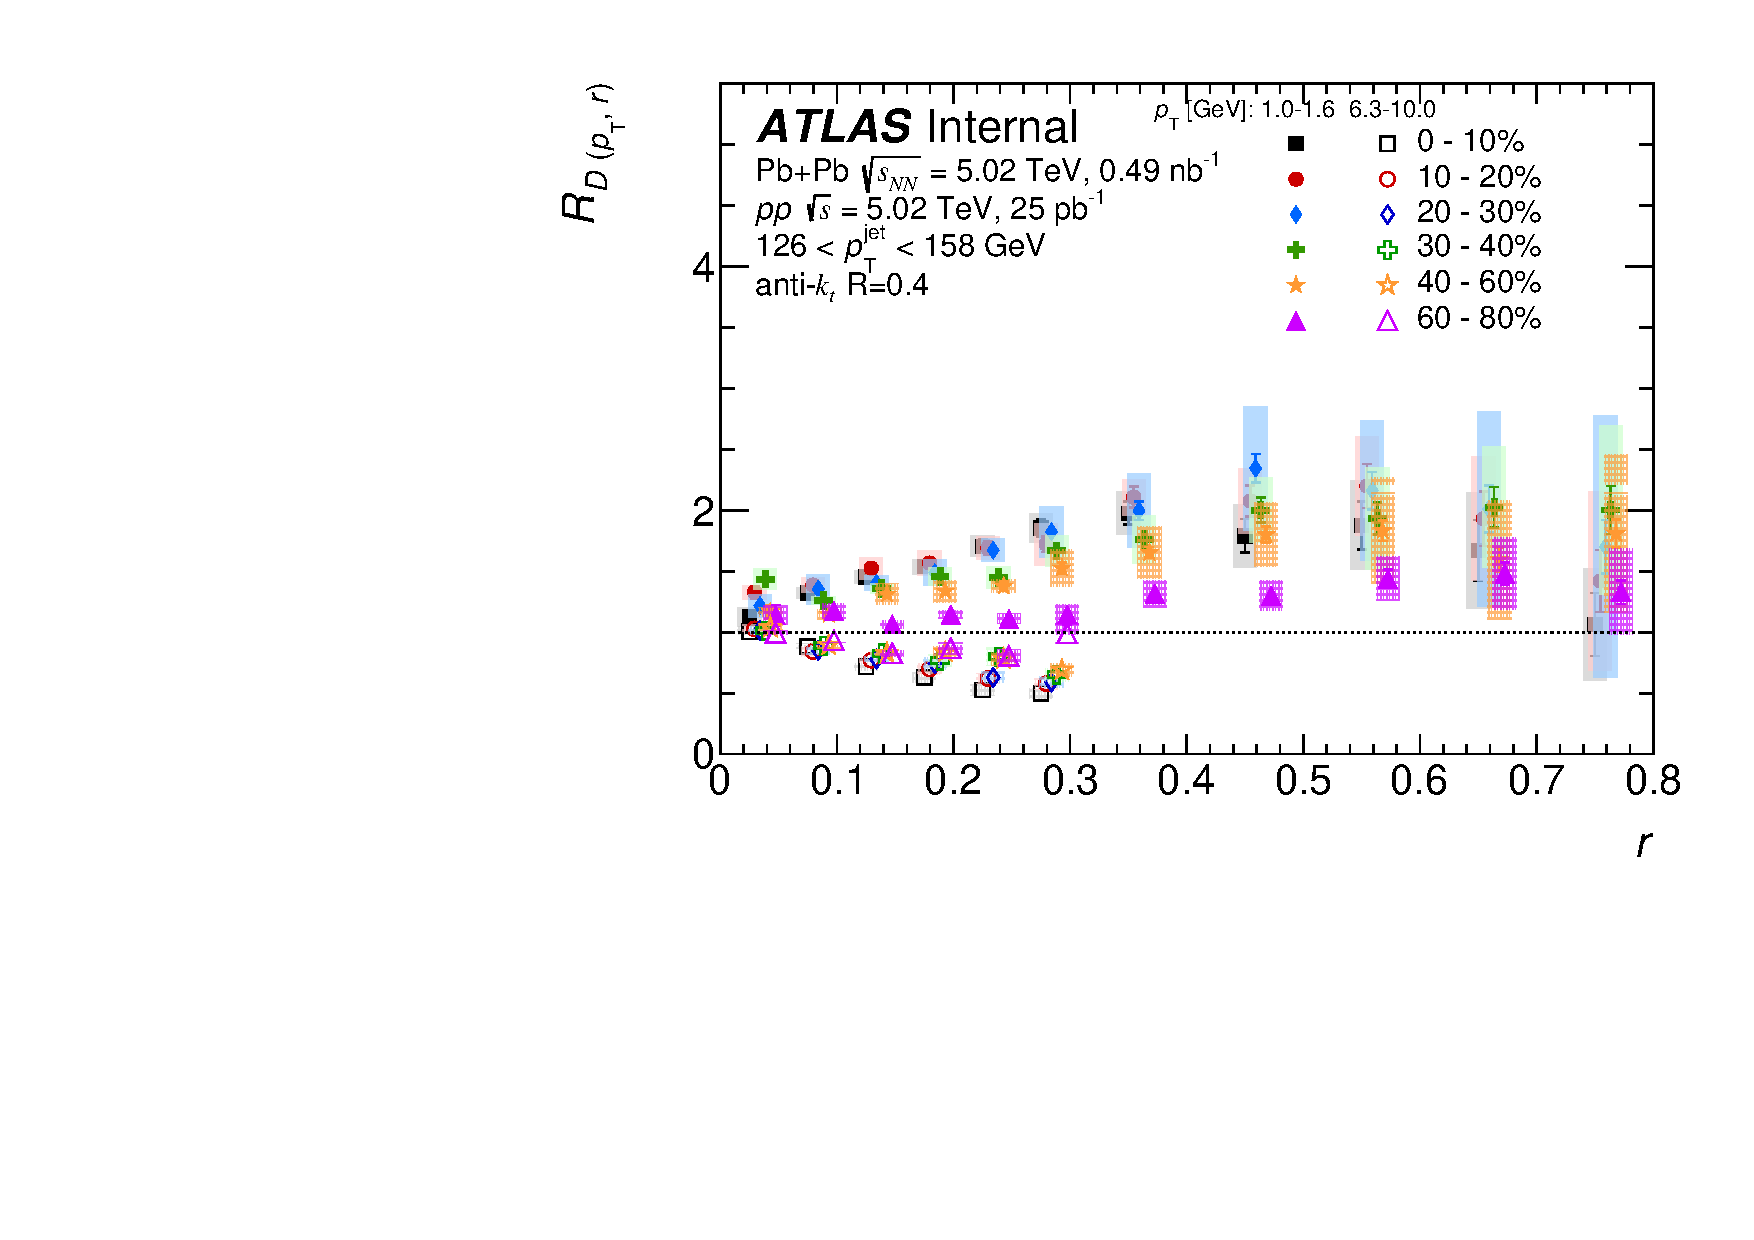
\includegraphics[width=0.5\textwidth]{figures/results/RDpT_dR_trk2_trk6_jet7.pdf} & 
            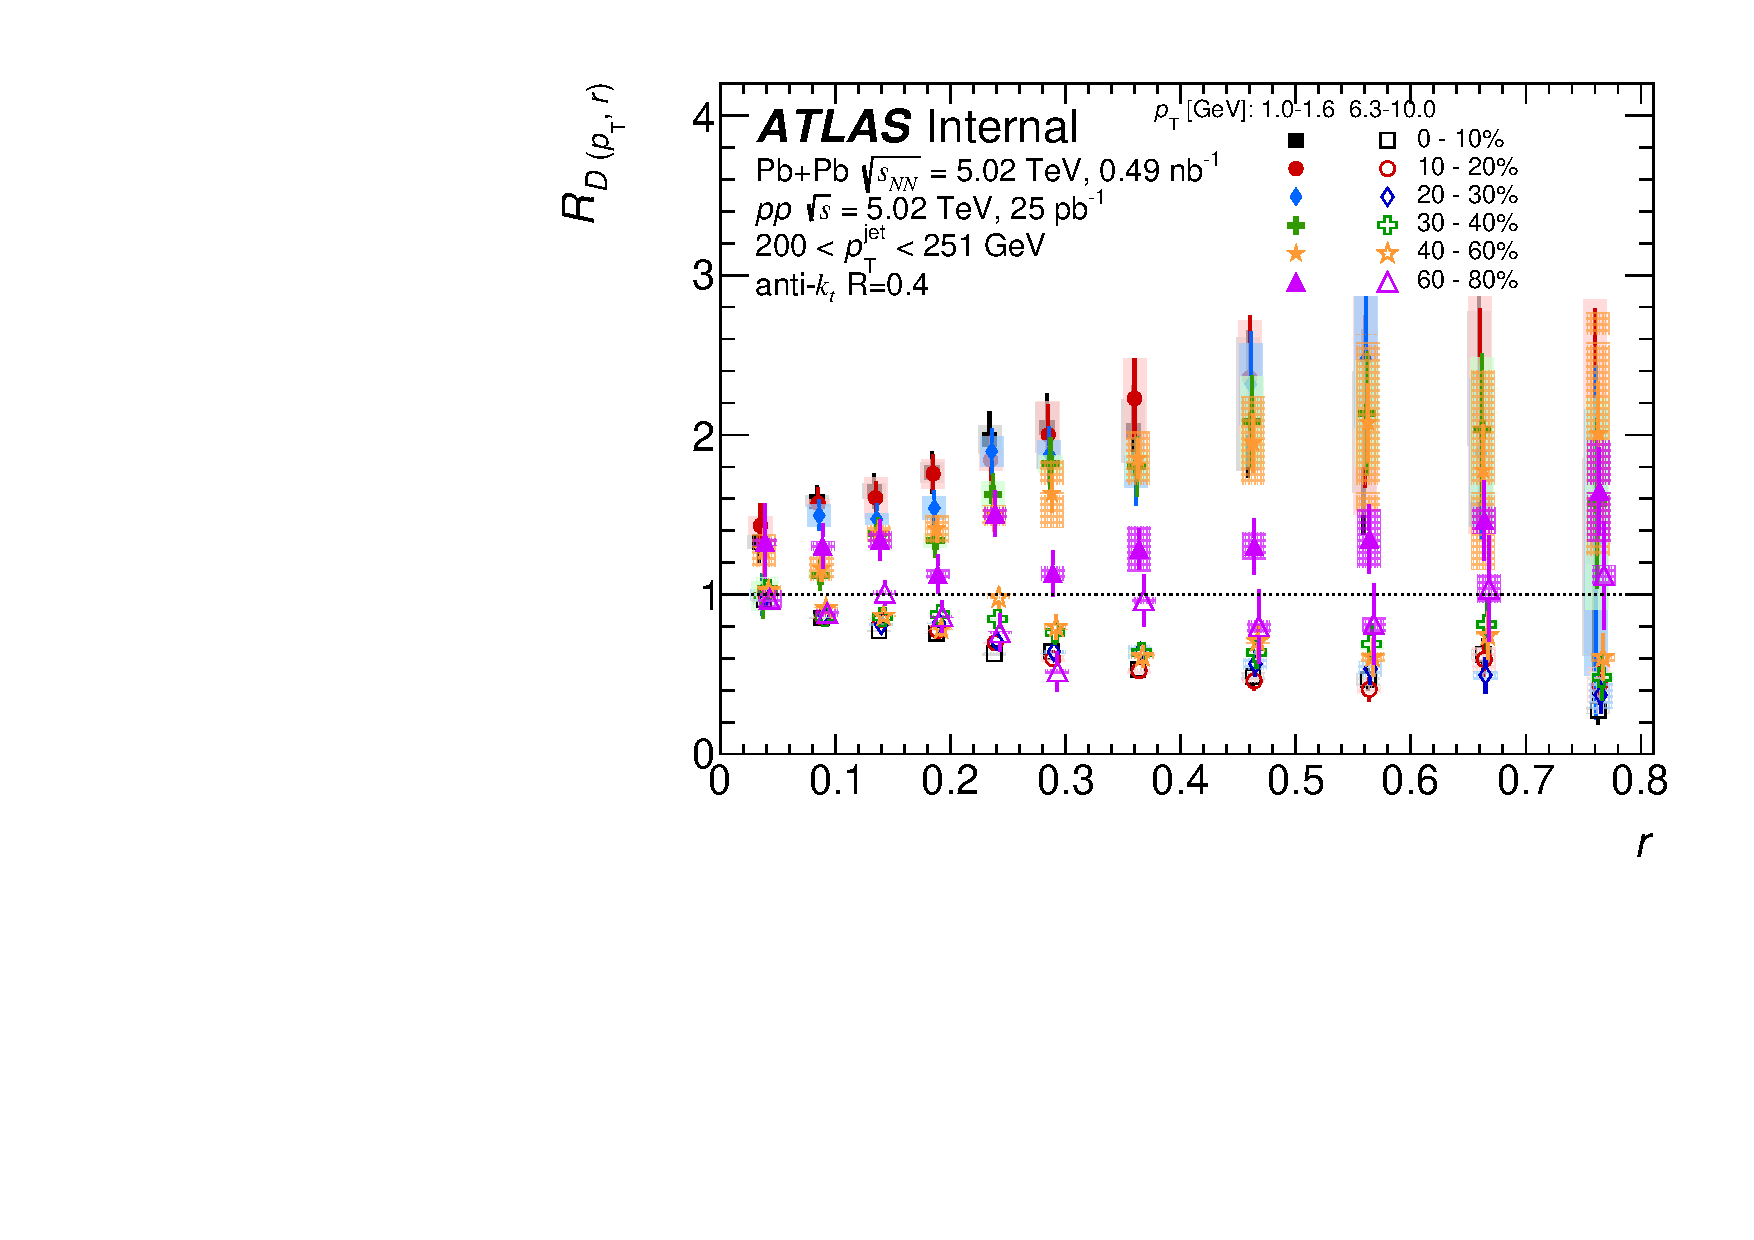
\includegraphics[width=0.5\textwidth]{figures/results/RDpT_dR_trk2_trk6_jet9.pdf} \\
      \end{tabular}
      }
\caption{The \RDptr\ distributions for \ptjet\ of 126--158~\GeV\ and 200--251~\GeV\ as a function of angular distance $r$ for two \pt\ selections and six centrality intervals (\pt\ selections are shown by closed and open symbols). The vertical bars on the data points indicate statistical uncertainties while the shaded boxes indicate systematic uncertainties. The widths of the boxes are not indicative of the bin size and the points are shifted horizontally for better visibility.}
\label{fig:centdep}
\end{figure}
%%%%%%%%%%%%%

%%pt jet dependence

\begin{figure}[ht]
\centerline{
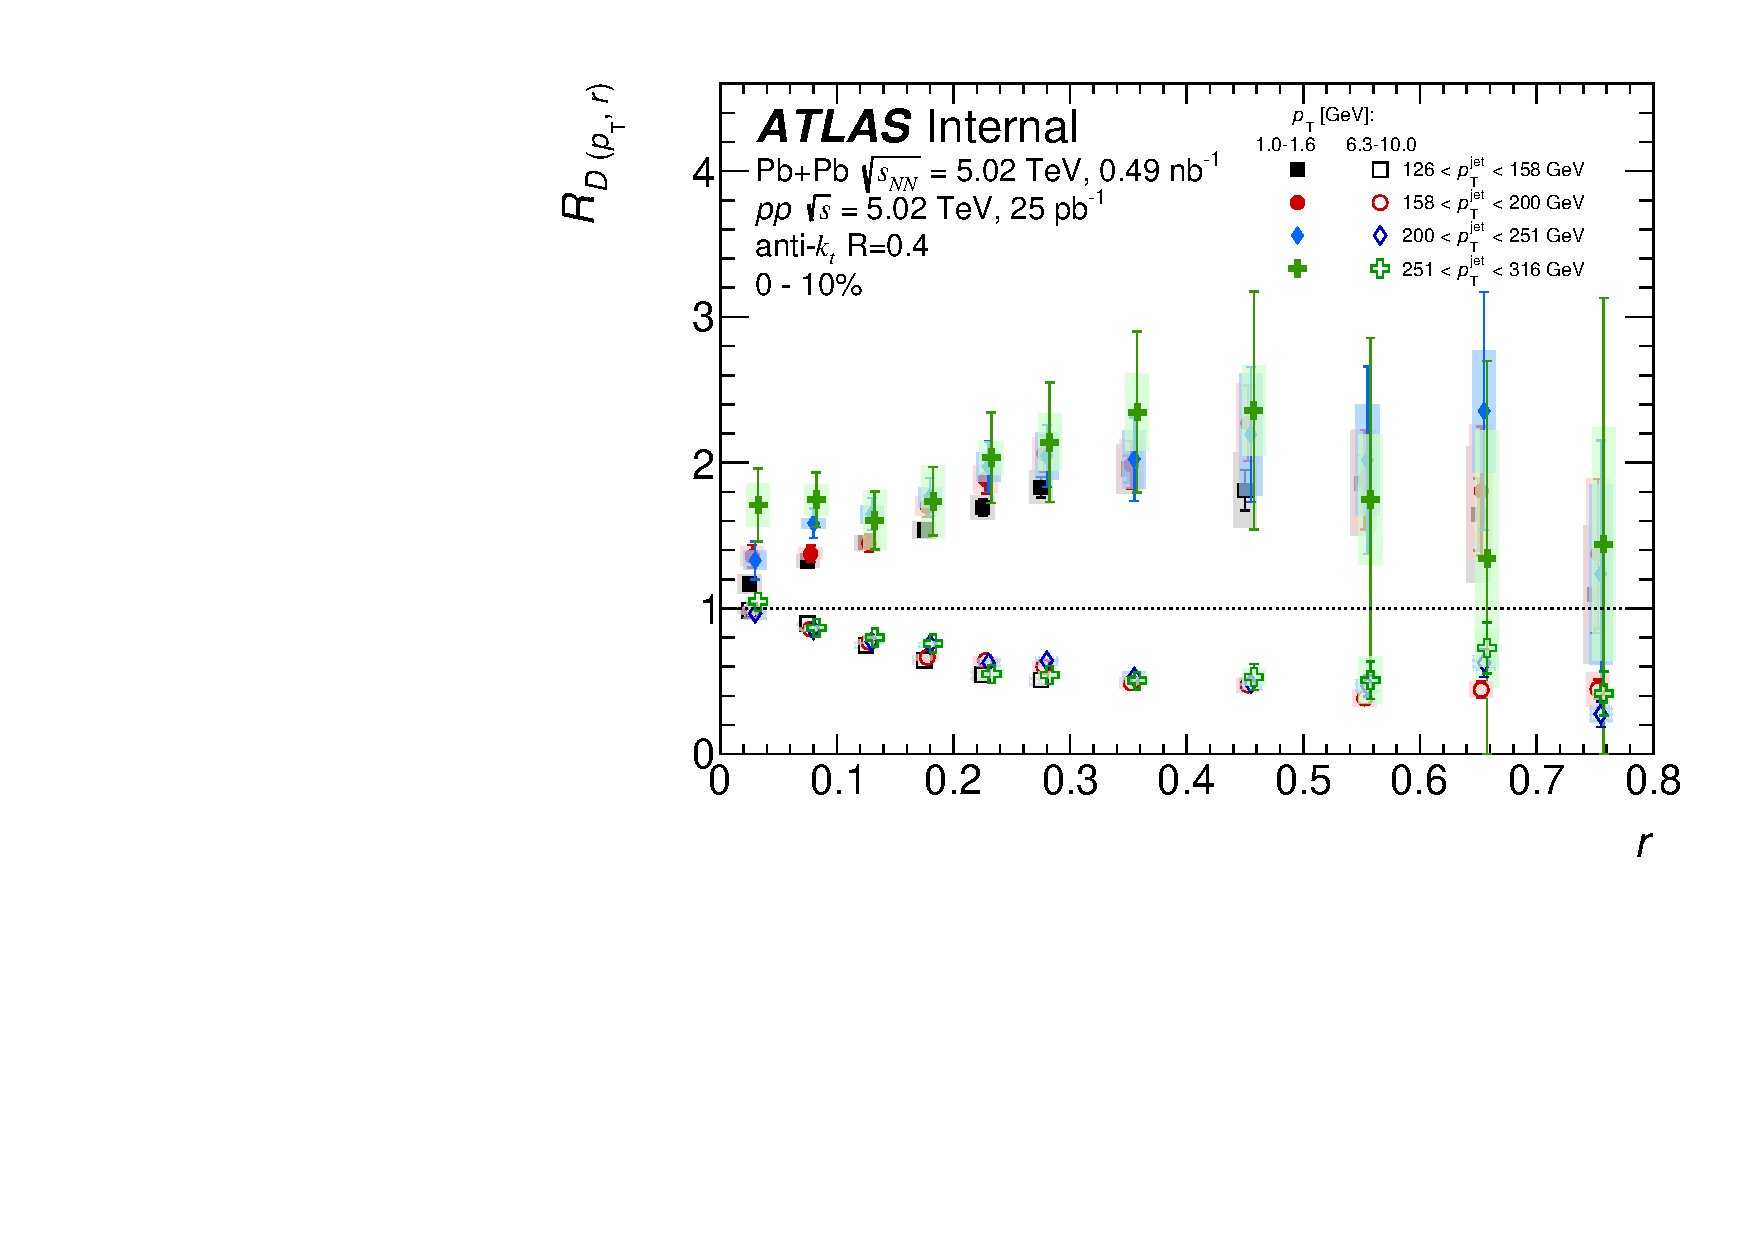
\includegraphics[width=0.8\textwidth]{figures/results/RDpT_dR_trk2_trk6_cent0.pdf} 
}
\caption{\RDptr\ as a function of \rvar\ for 0--10\% collisions for charged particles with 1.0~$< \pt <$~1.6~\GeV\
(closed symbols) and 6.3~$< \pt <$10.0~\GeV\ (open symbols) for different \ptjet\ selections. The vertical bars on the data points indicate statistical uncertainties while the shaded boxes indicate systematic uncertainties. The widths of the boxes are not indicative of the bin size and the points are shifted horizontally for better visibility.}
\label{fig:ptjetdep}
\end{figure}
%%%%%%%%%%%%%


%%pt track dependence
The charged particle \pt\ dependence of \RDptr\ for \mbox{$126 < \ptjet < 158$ GeV} and \mbox{$200 < \ptjet < 251$ GeV}, at a variety of angular distances from the jet axis in 0--10\% central and 60--80\% peripheral collisions is presented in Figure~\ref{fig:pttrkdep}. No suppression is observed for $r < 0.05$ across the entire \pt\ range under investigation. This can also be seen in Figure~\ref{fig:rdptr} and Figure~\ref{fig:rdptr_trk_cent}, where any suppression in the charged particle spectra is at distances larger than $r = 0.05 $ 
from the jet axis. 

\begin{figure}
\centering{
\begin{tabular}{cc}
	 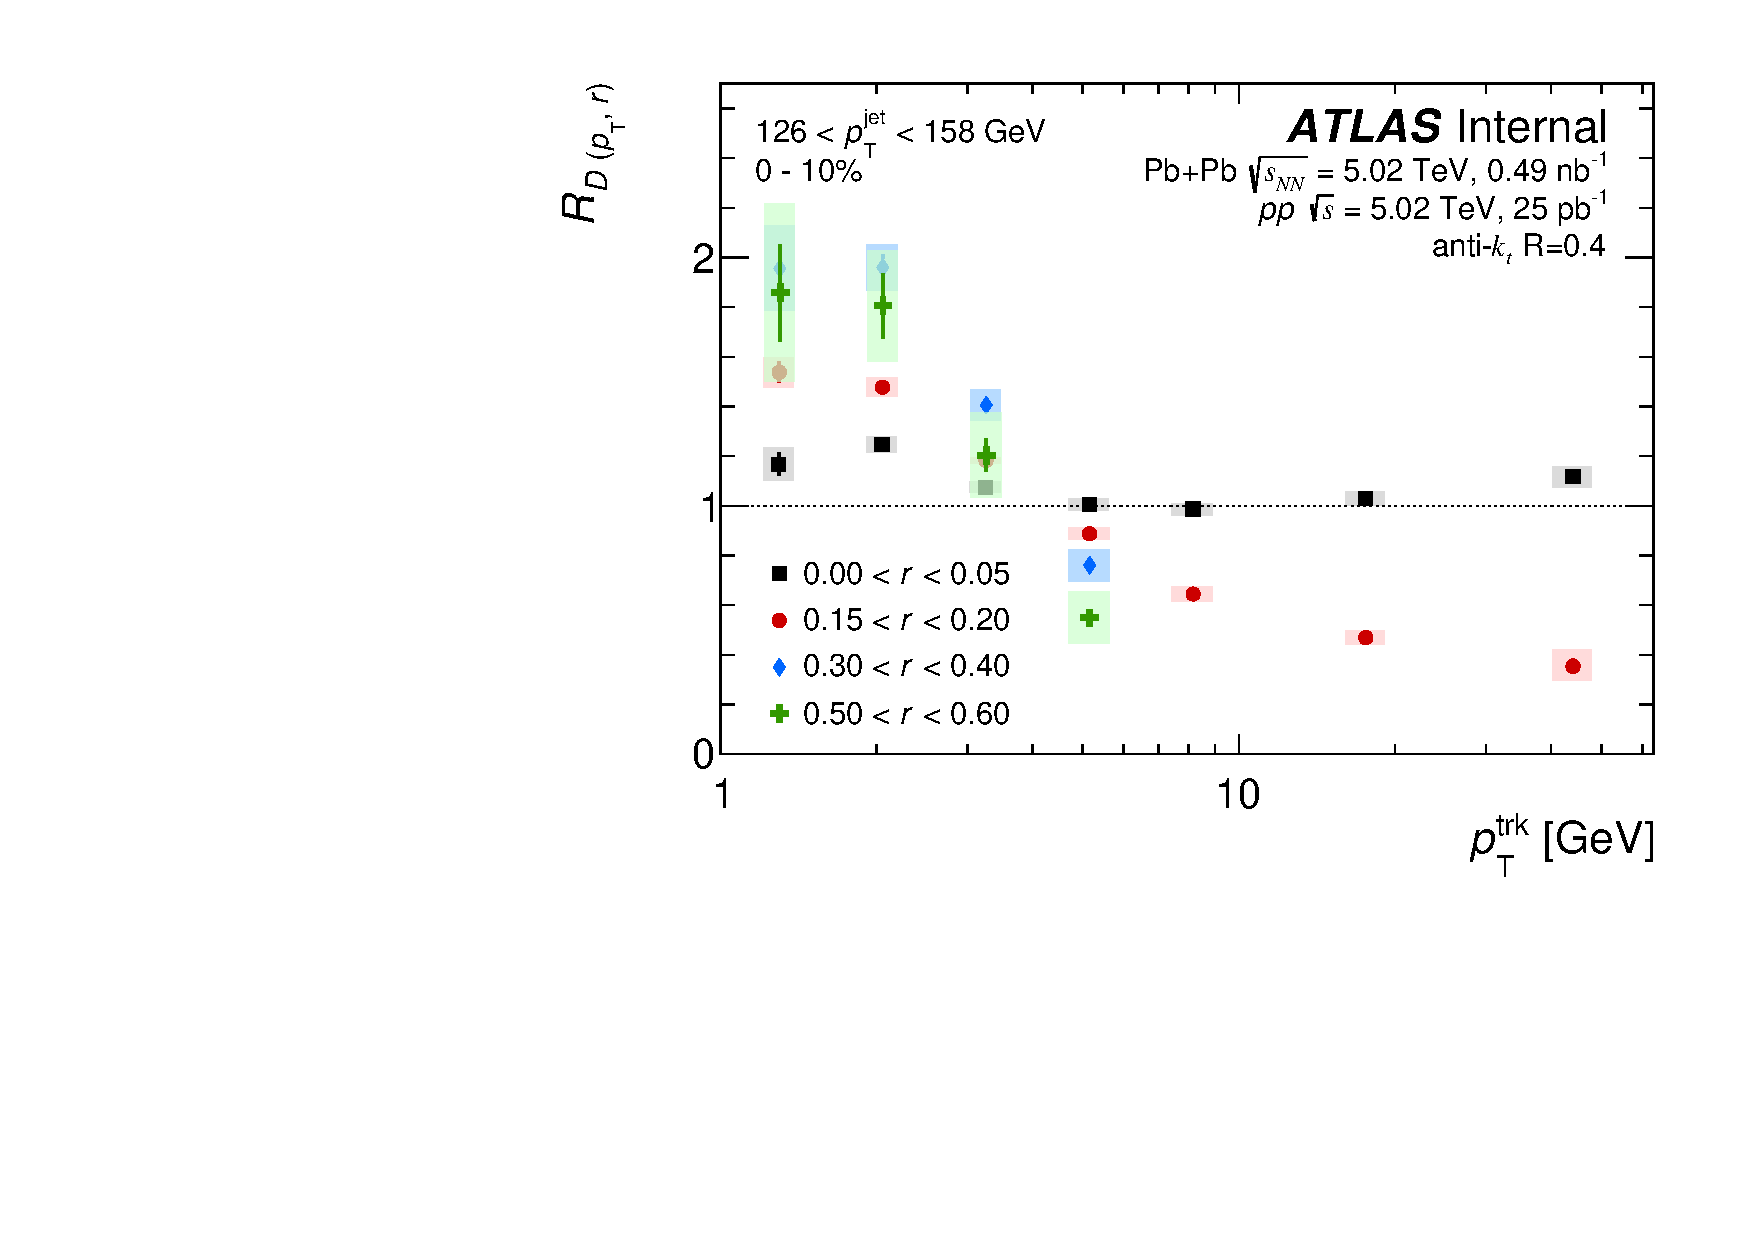
\includegraphics[width=0.5\textwidth]{results/RDpT_trkpt_jet7_cent0} &
	 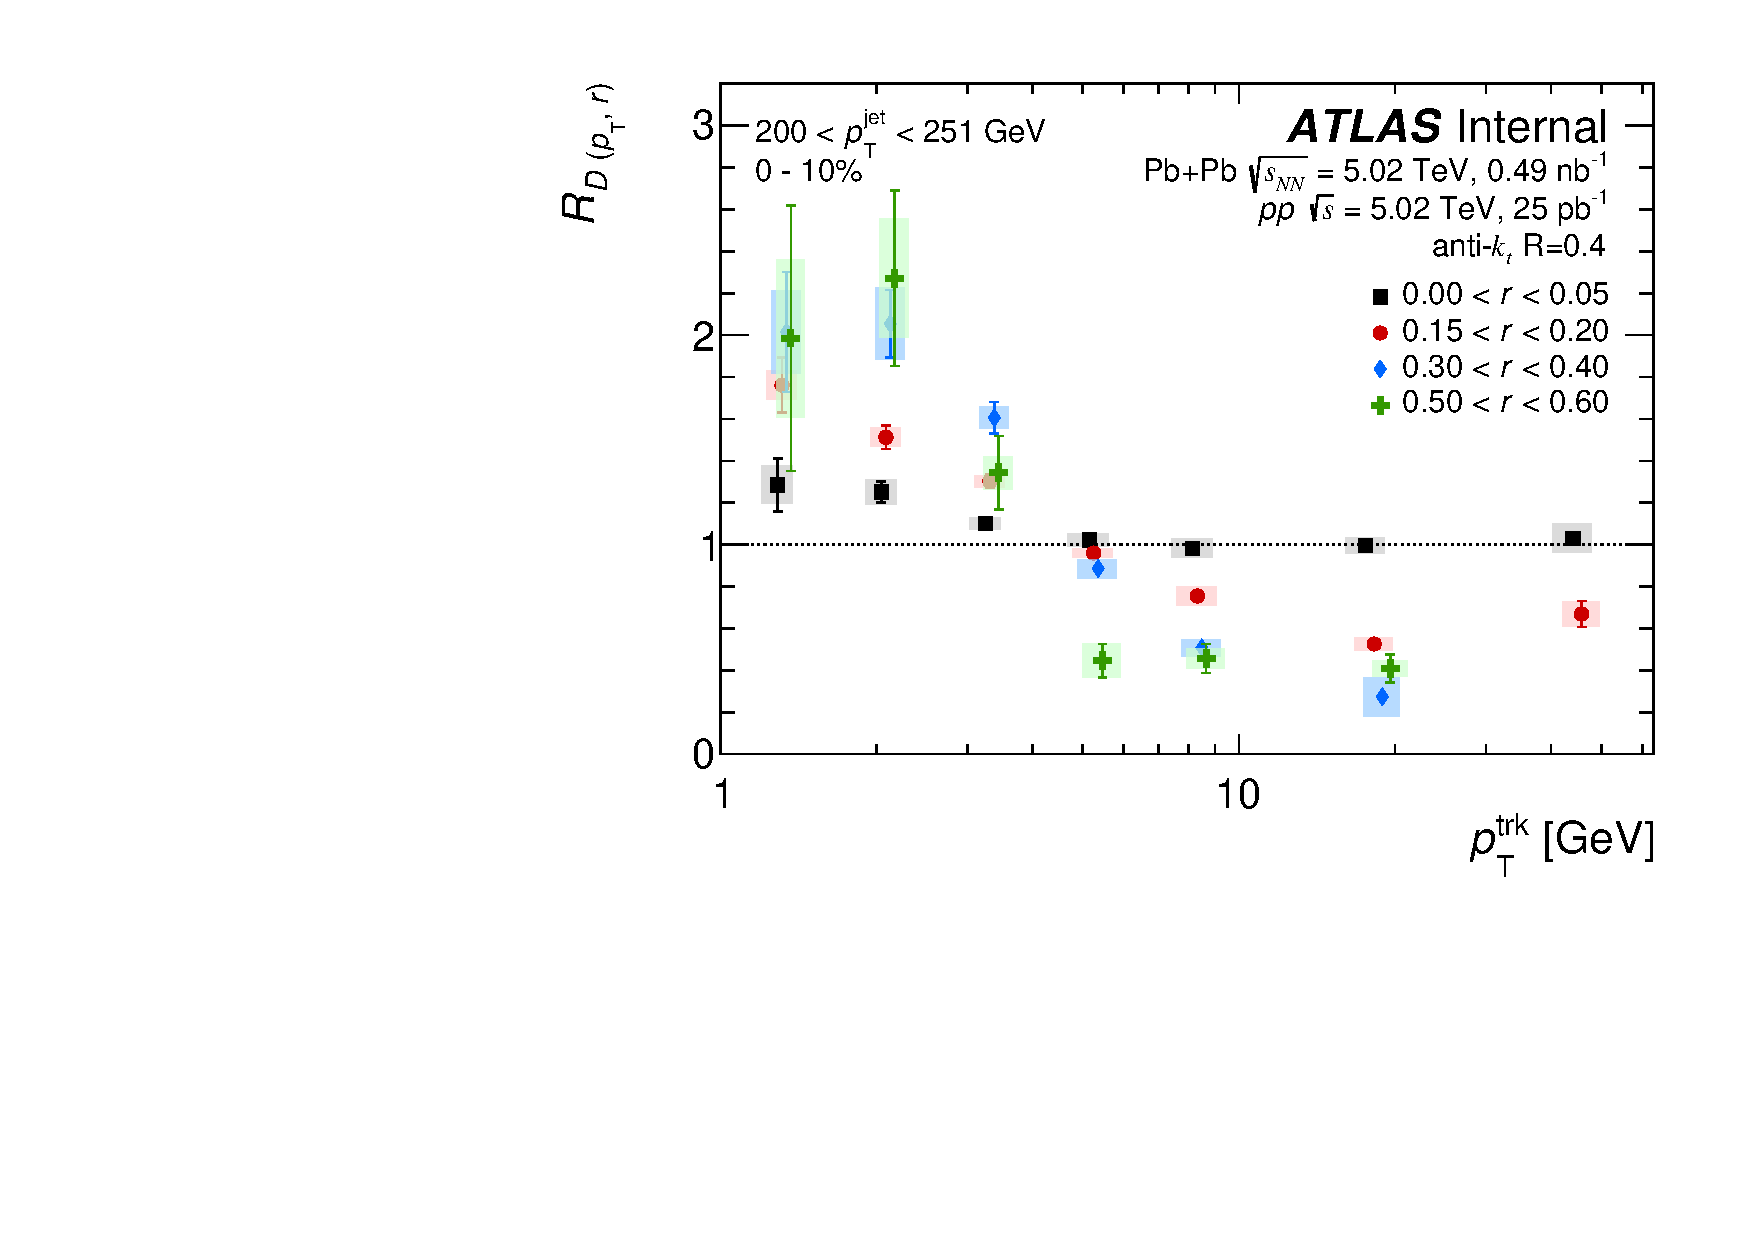
\includegraphics[width=0.5\textwidth]{results/RDpT_trkpt_jet9_cent0} \\
	 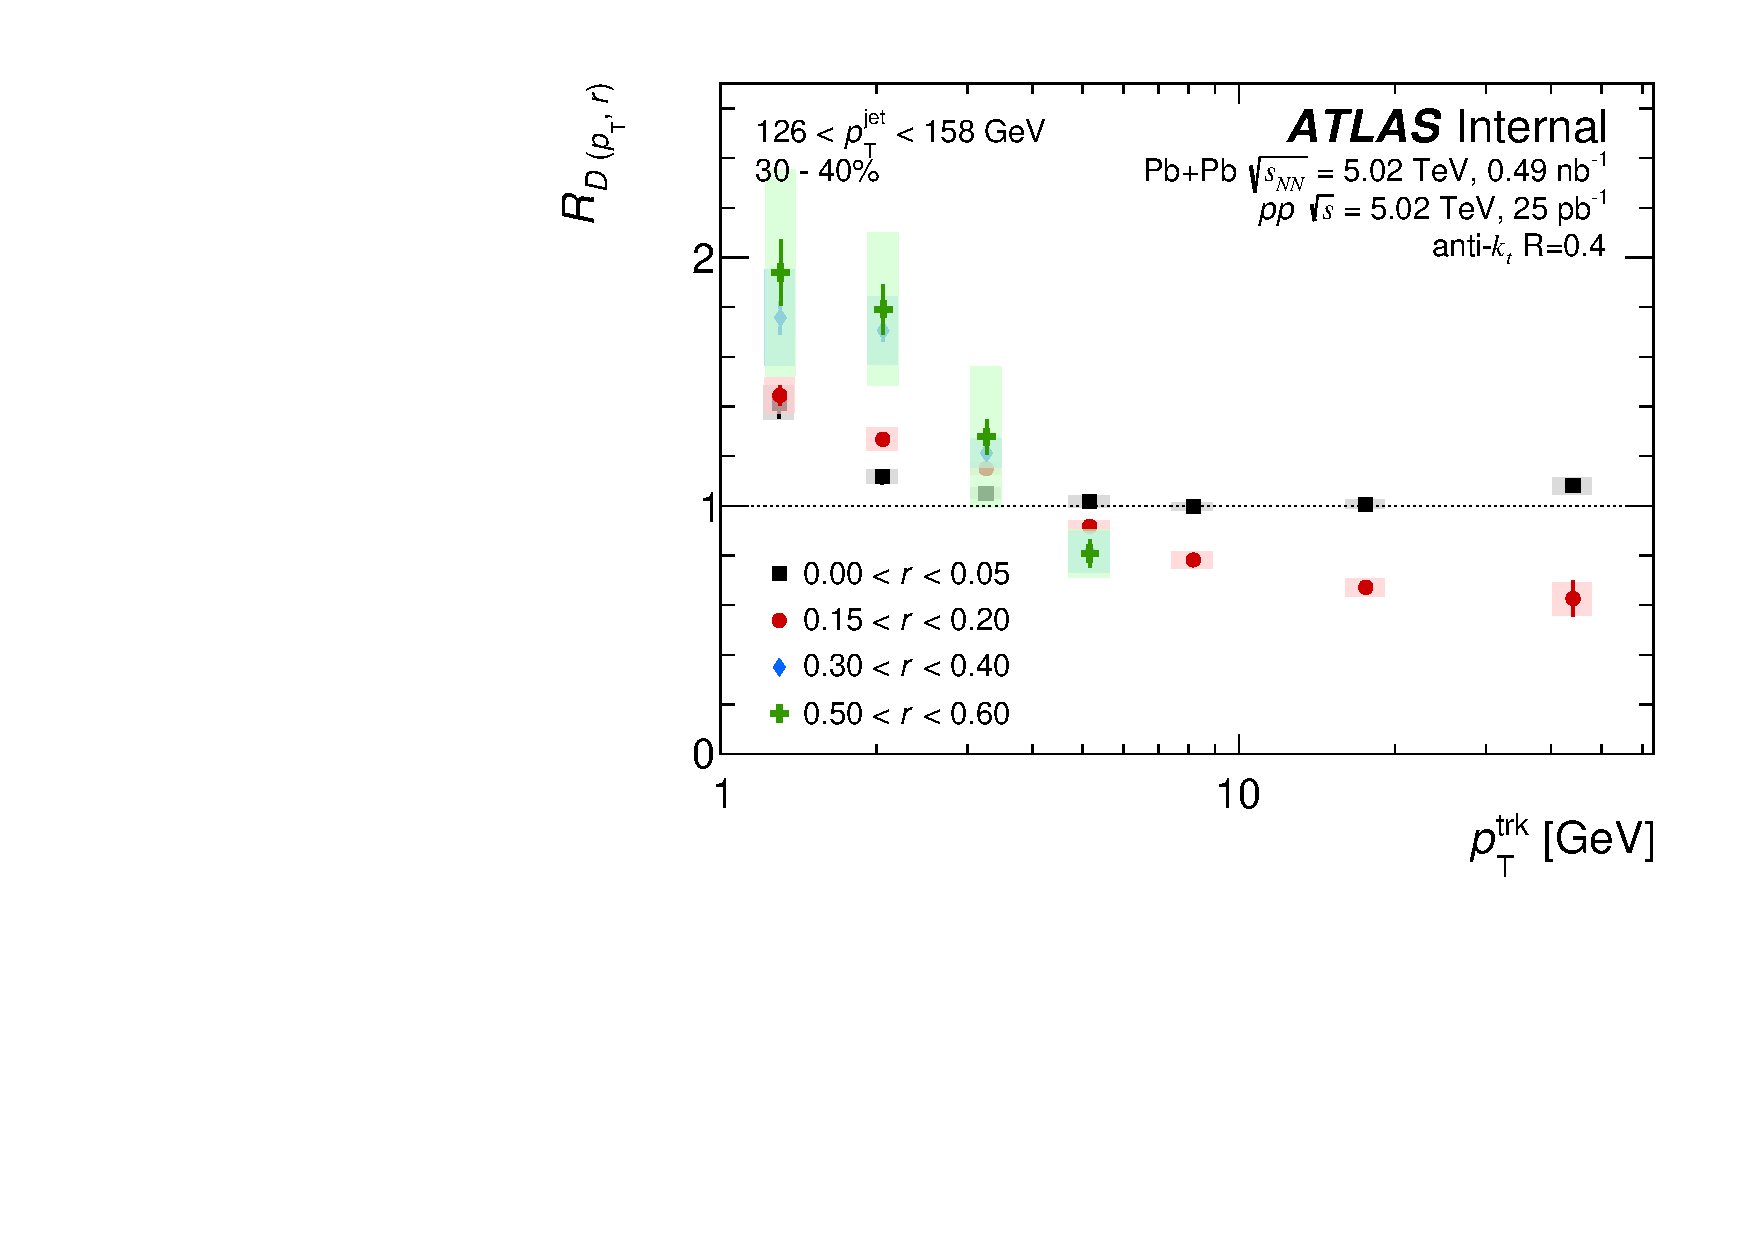
\includegraphics[width=0.5\textwidth]{results/RDpT_trkpt_jet7_cent3} &
	 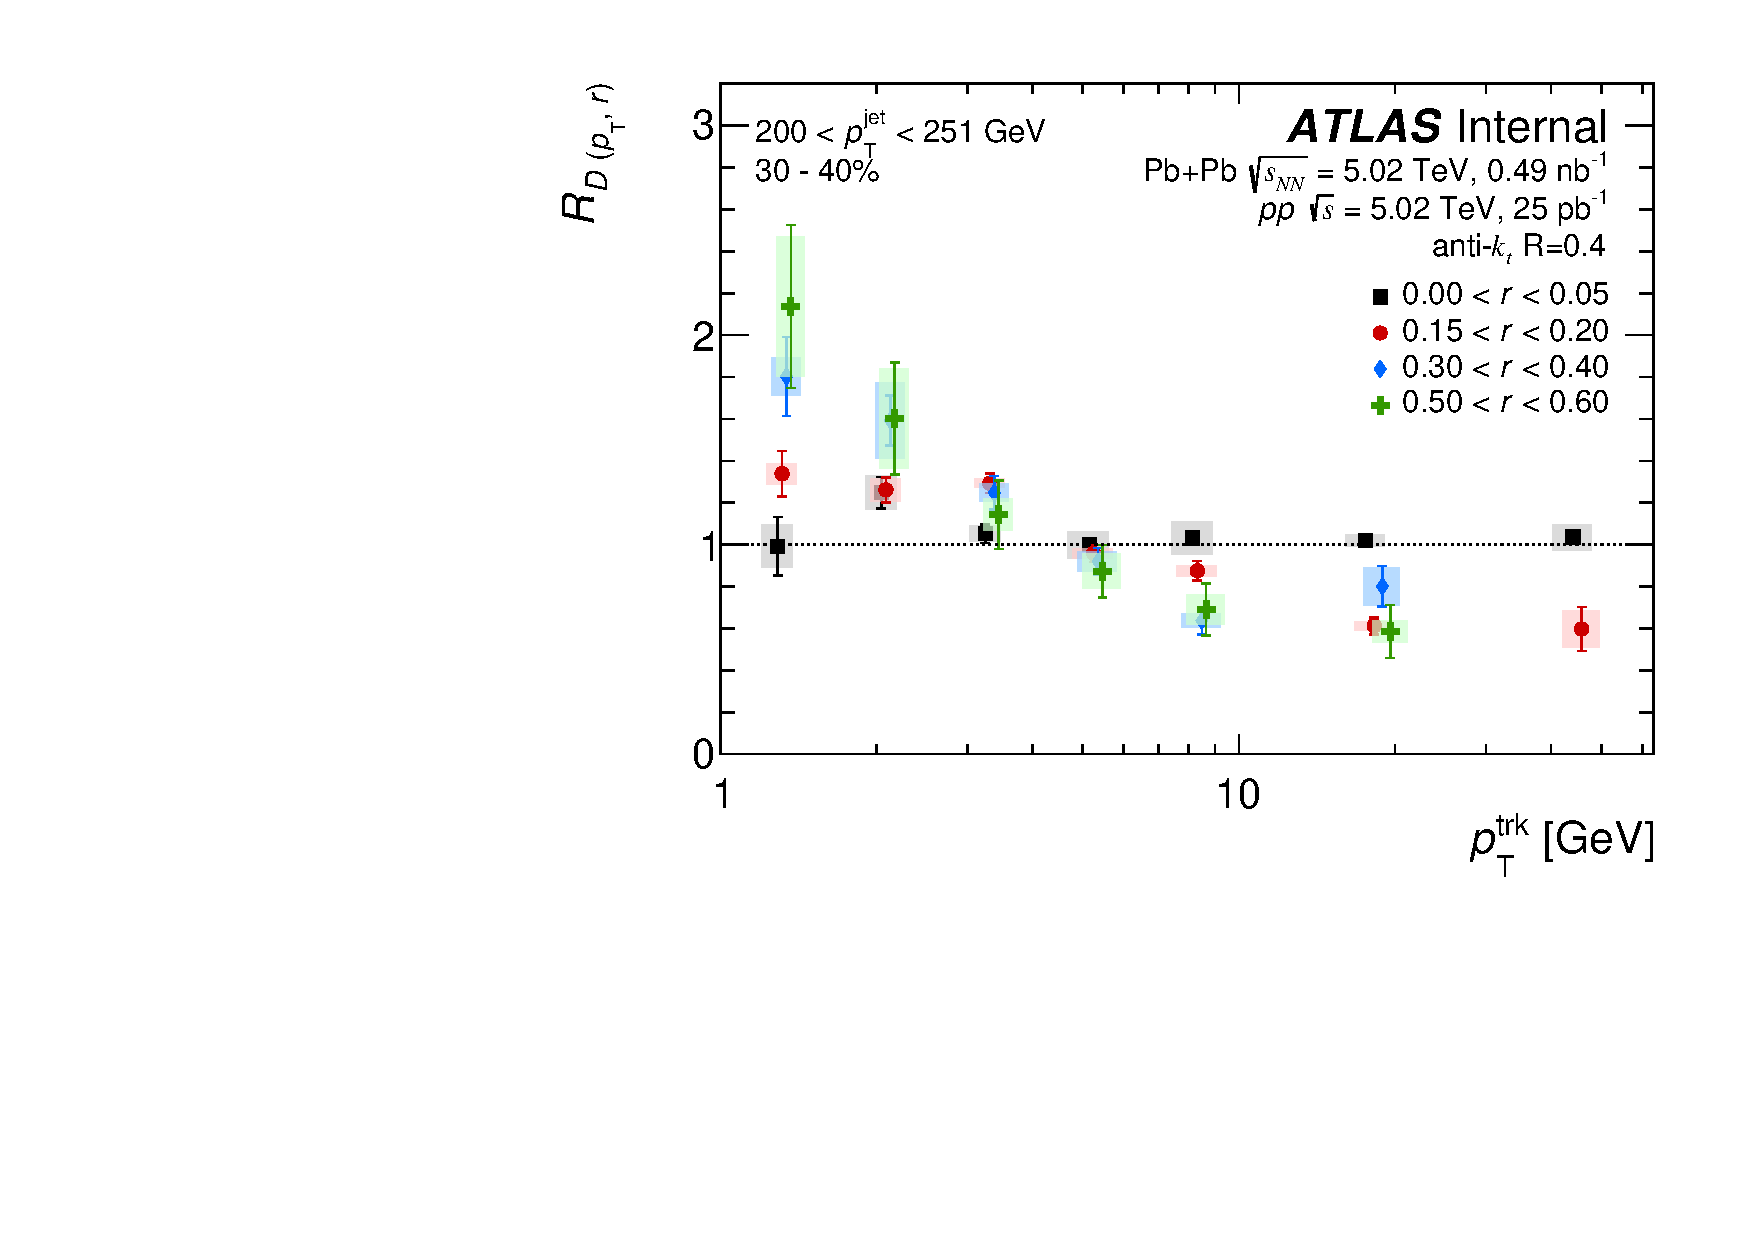
\includegraphics[width=0.5\textwidth]{results/RDpT_trkpt_jet9_cent3} \\
	 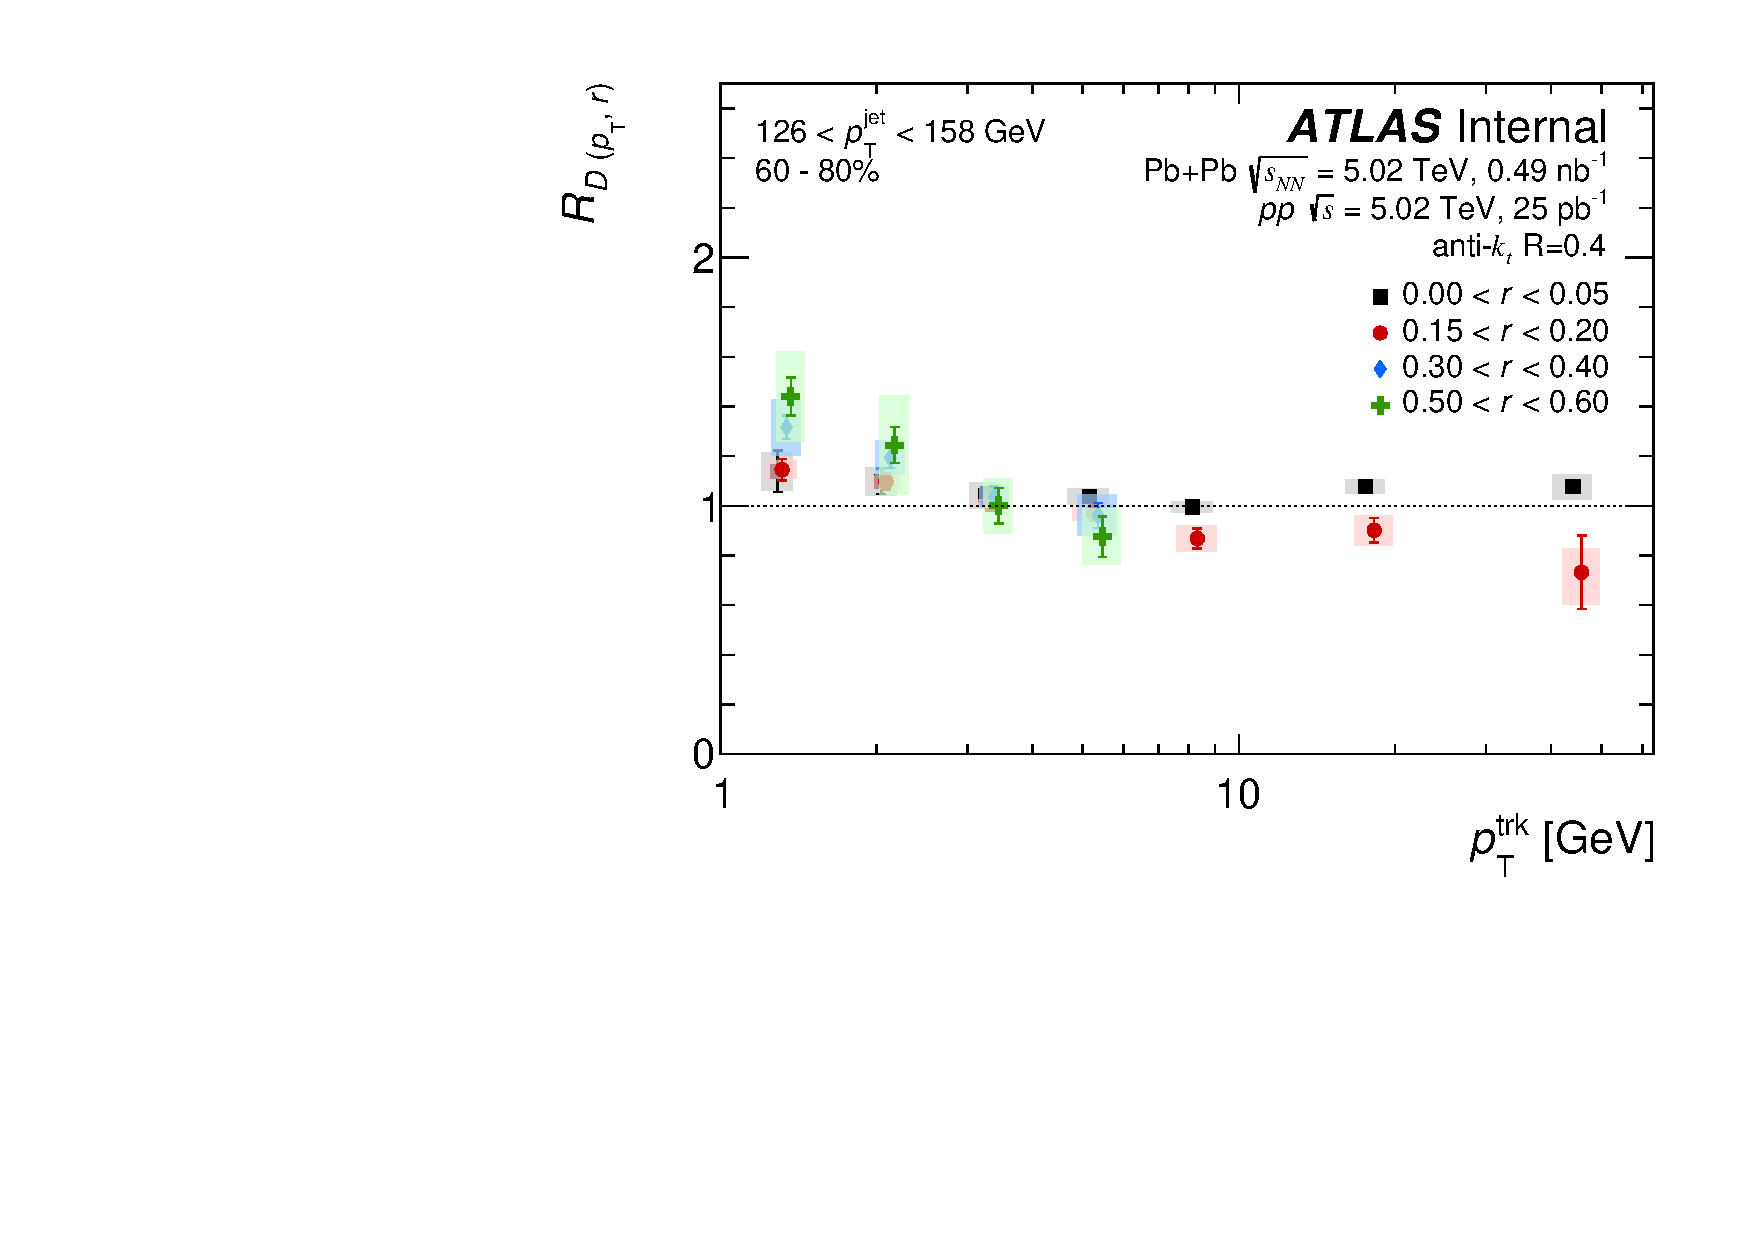
\includegraphics[width=0.5\textwidth]{results/RDpT_trkpt_jet7_cent5} &
	 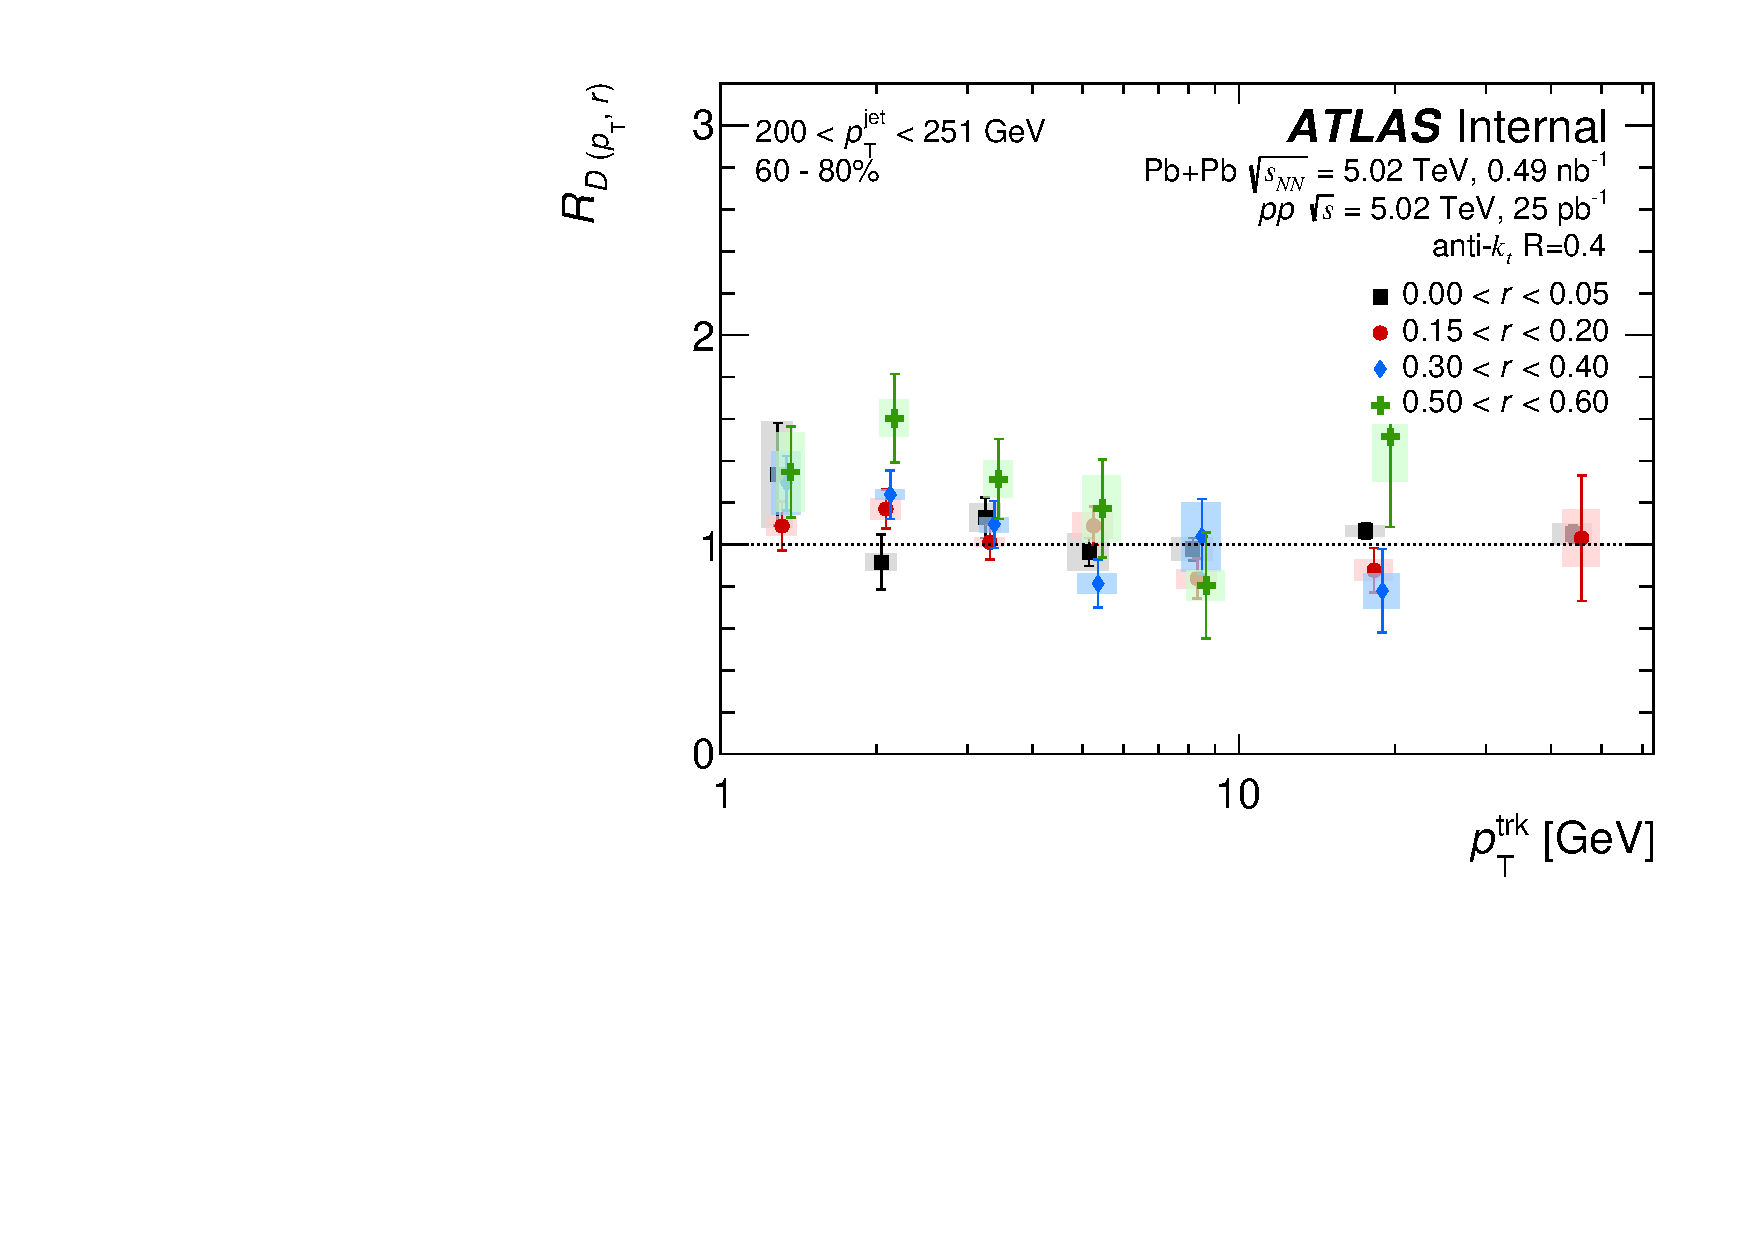
\includegraphics[width=0.5\textwidth]{results/RDpT_trkpt_jet9_cent5} \\
\end{tabular} }
   \caption{\RDptr\ as a function of \pt\ in  0--10\% (top), 30--40\% (middle), and 60--80\% (bottom) \PbPb\ collisions to \pp\ collisions for two different \ptjet\ selections: 126--158~\GeV\ (left) and 200--251~\GeV\ (right). The different colors indicate different angular distances from the jet axis. The vertical bars on the data points indicate statistical uncertainties while the shaded boxes indicate systematic uncertainties. The widths of the boxes are not indicative of the bin size and the points are shifted horizontally for better visibility.}
      \label{fig:pttrkdep}
\end{figure}

\begin{figure}
\centering{
\begin{tabular}{cc}
	 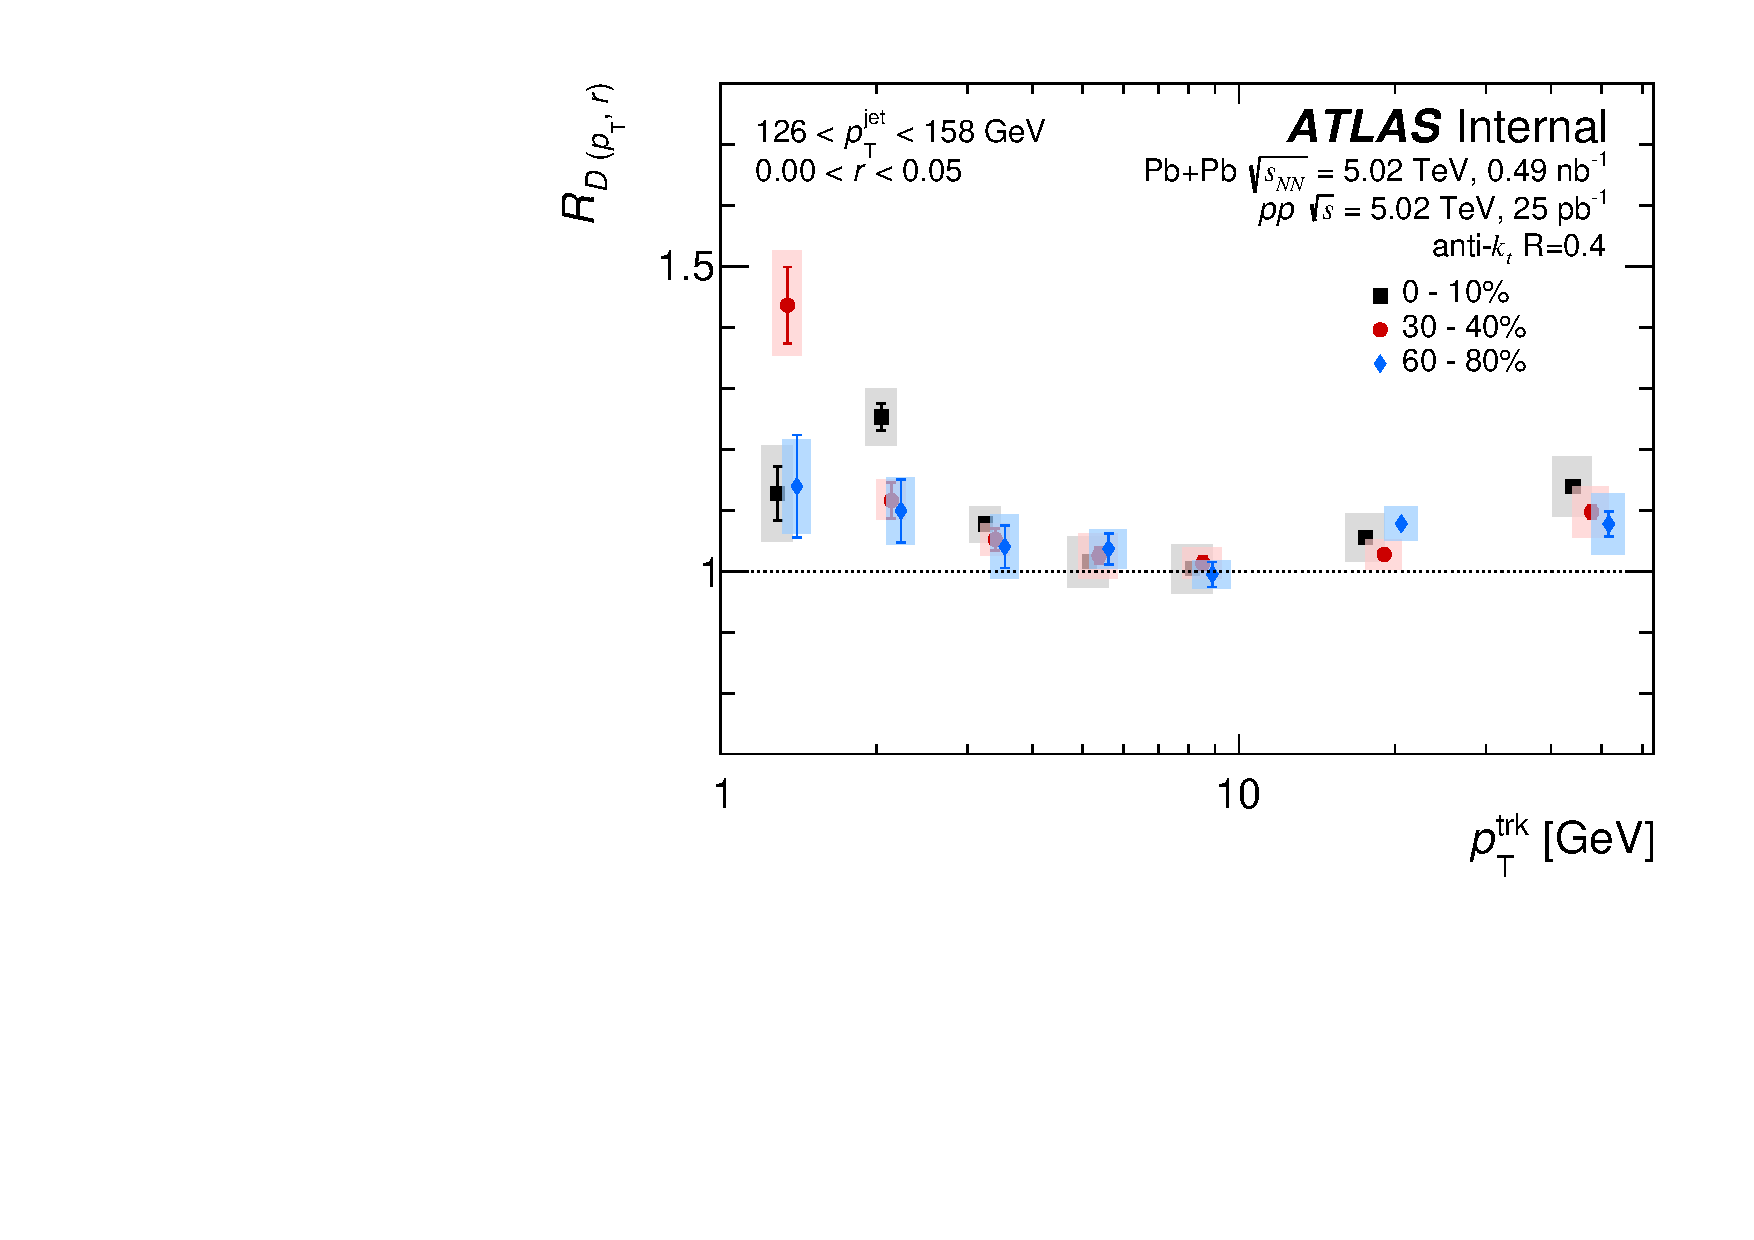
\includegraphics[width=0.5\textwidth]{results/RDpT_trkpt_jet7_dR0} &
	 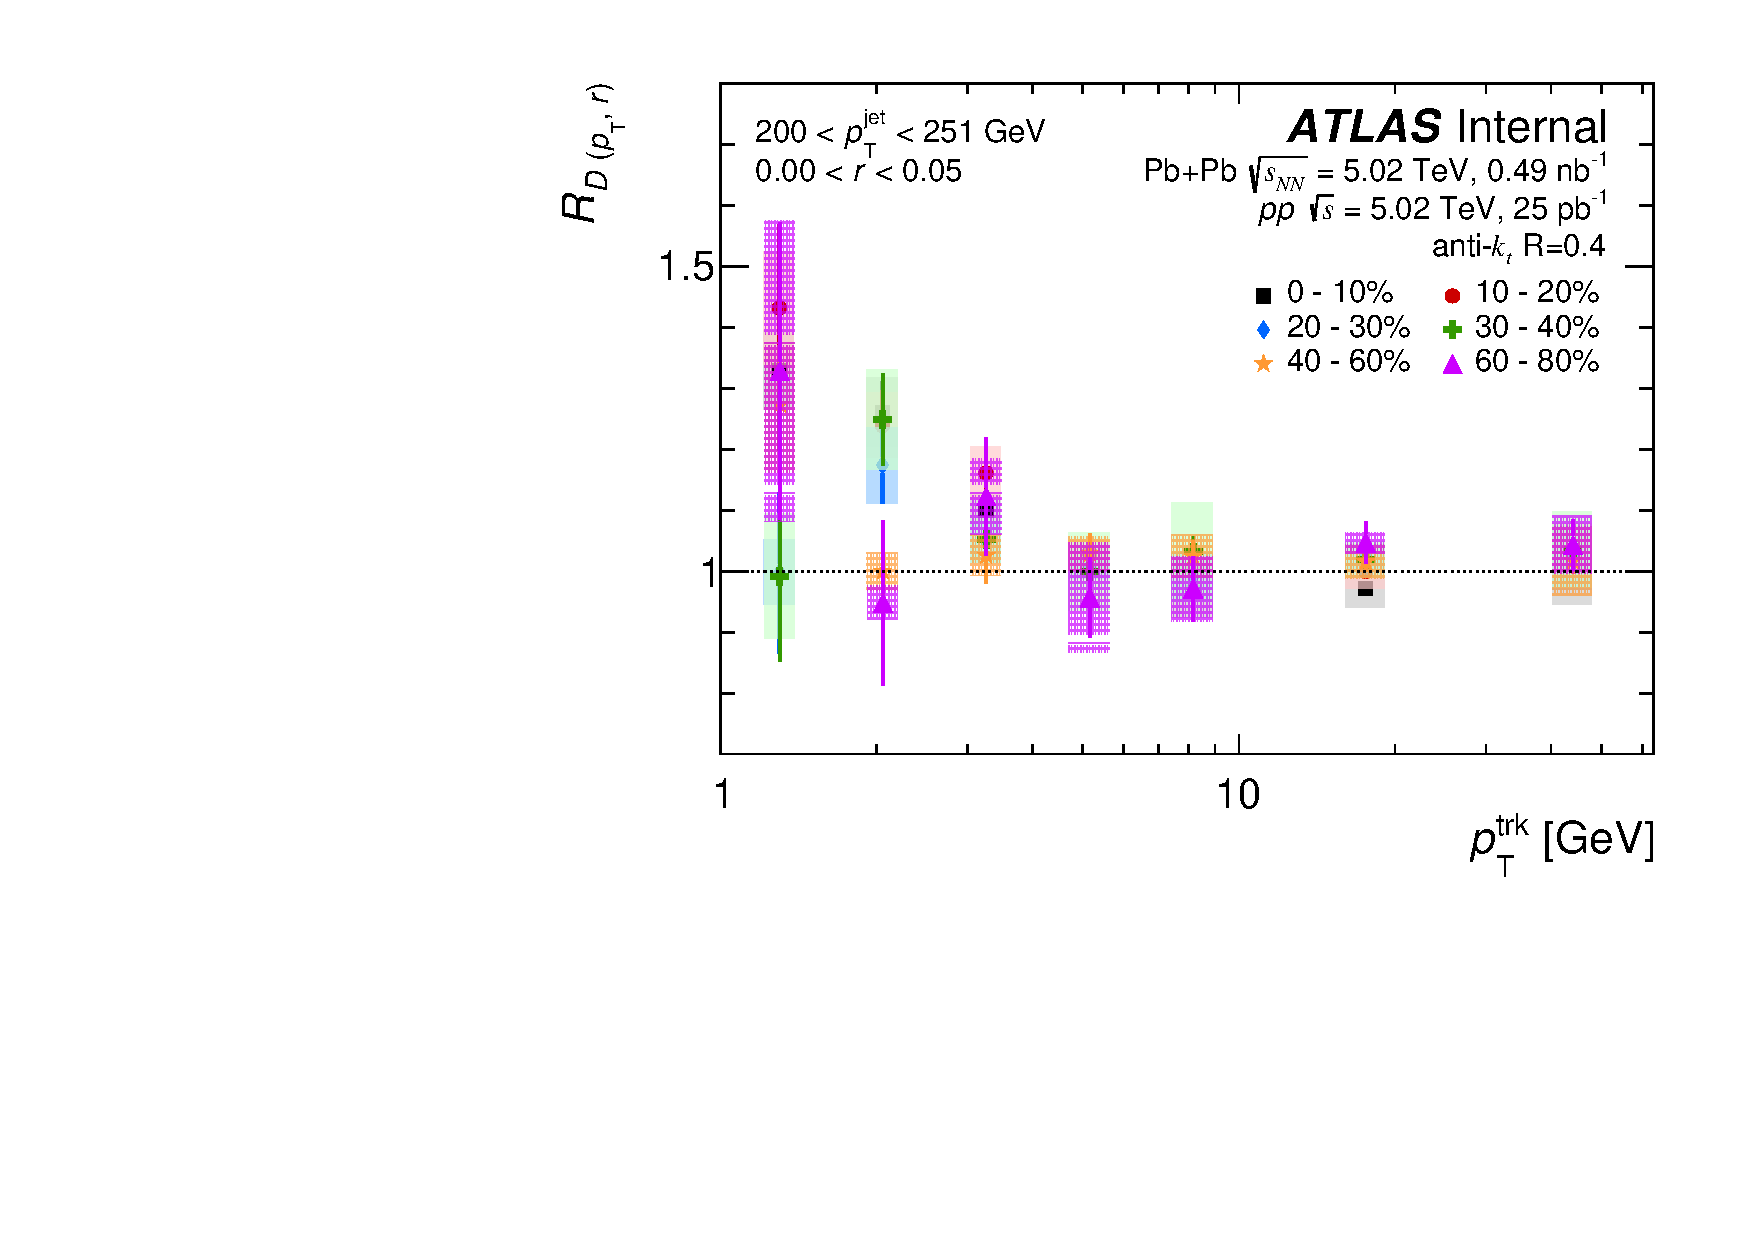
\includegraphics[width=0.5\textwidth]{results/RDpT_trkpt_jet9_dR0} \\
	 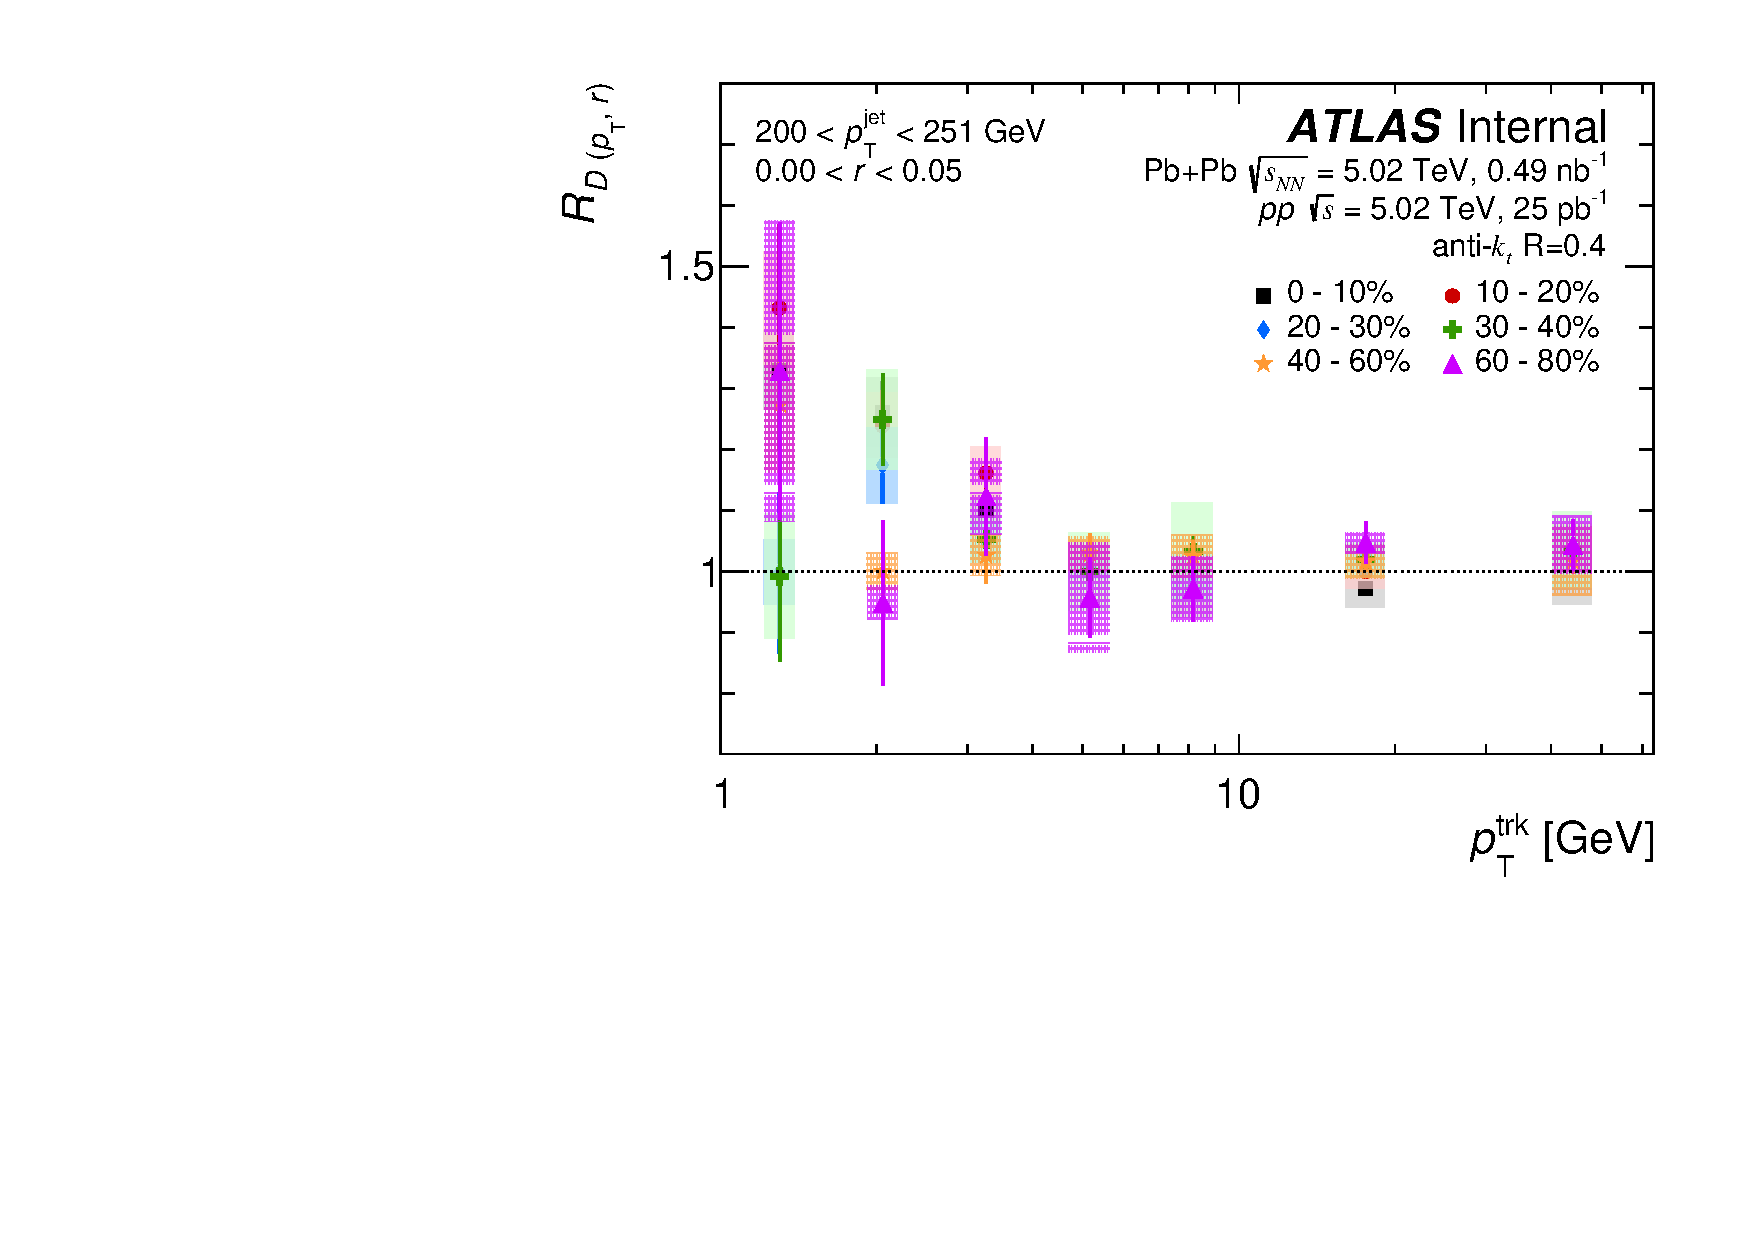
\includegraphics[width=0.5\textwidth]{results/RDpT_trkpt_jet9_dR0} &
	 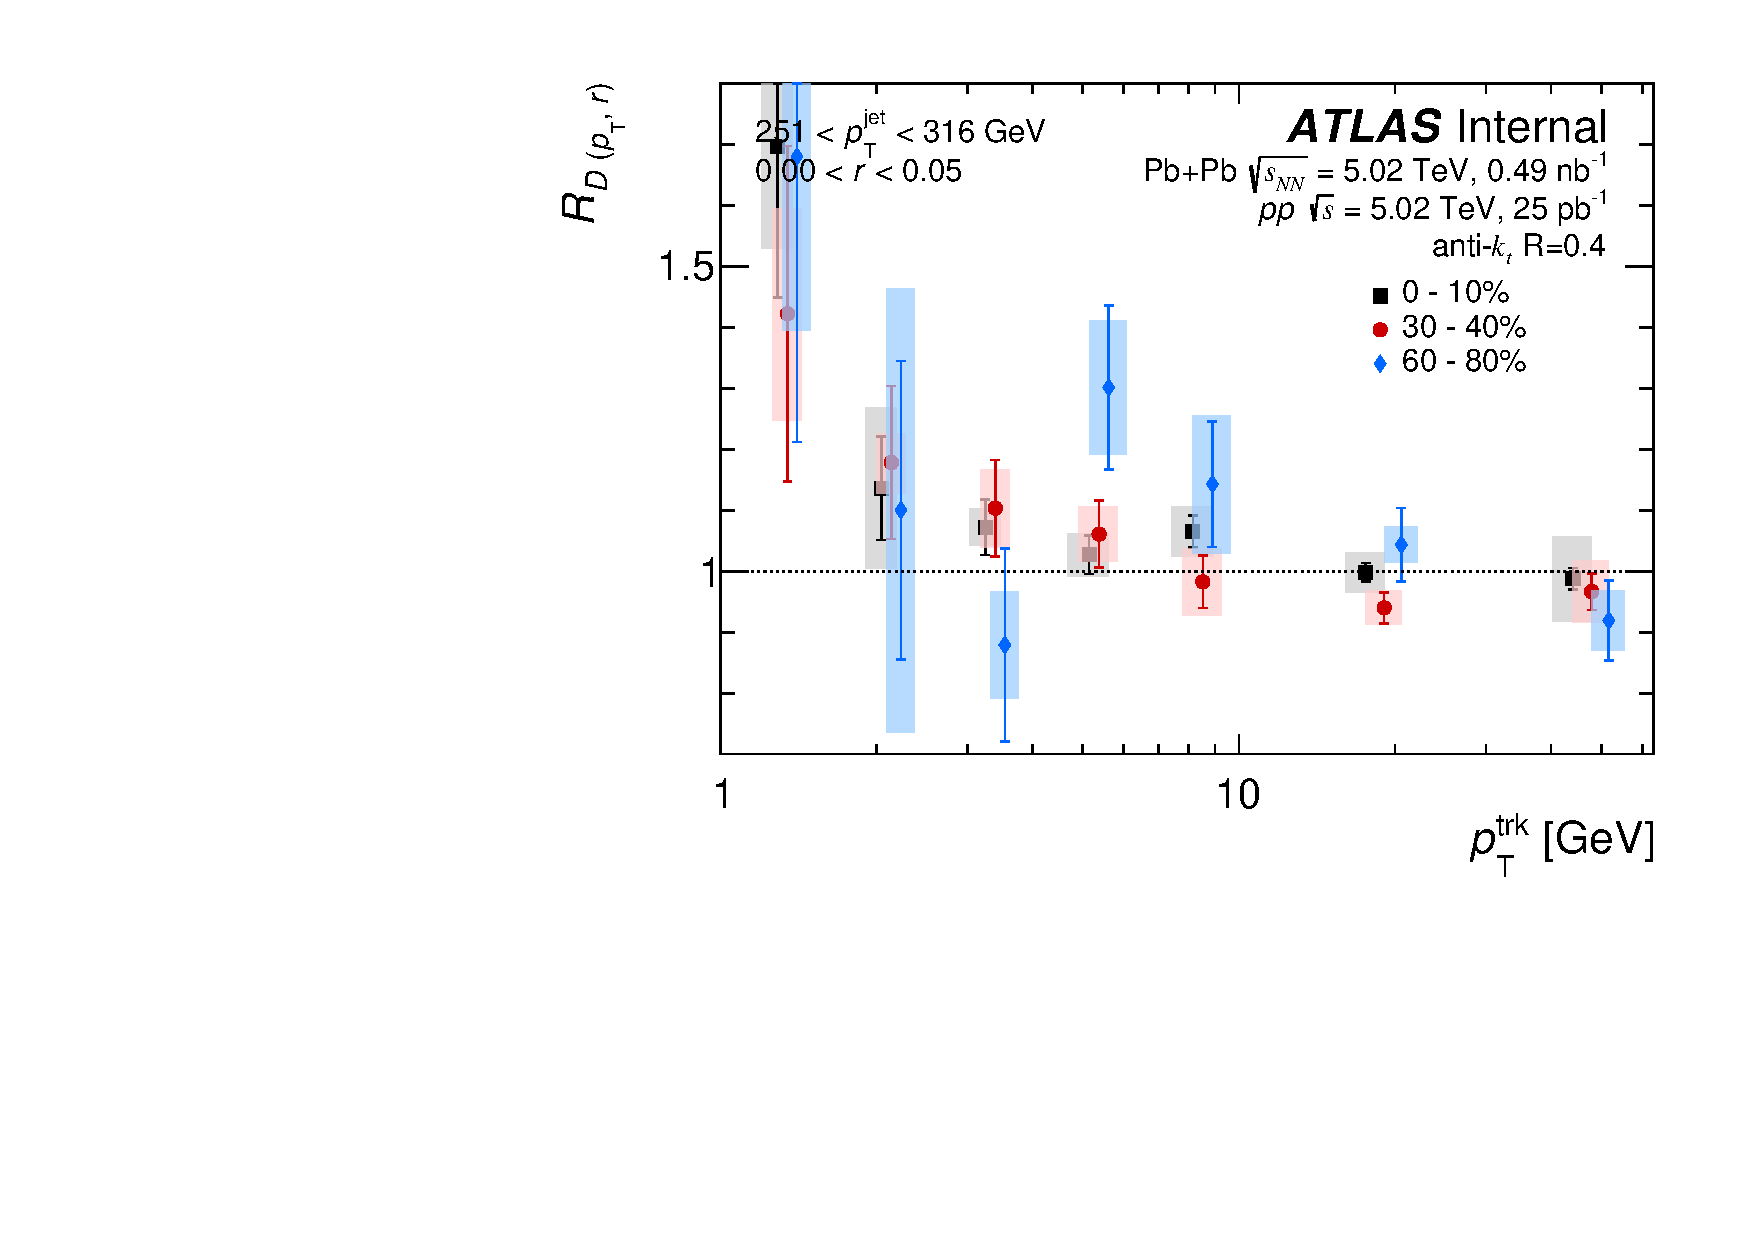
\includegraphics[width=0.5\textwidth]{results/RDpT_trkpt_jet10_dR0} \\
%	 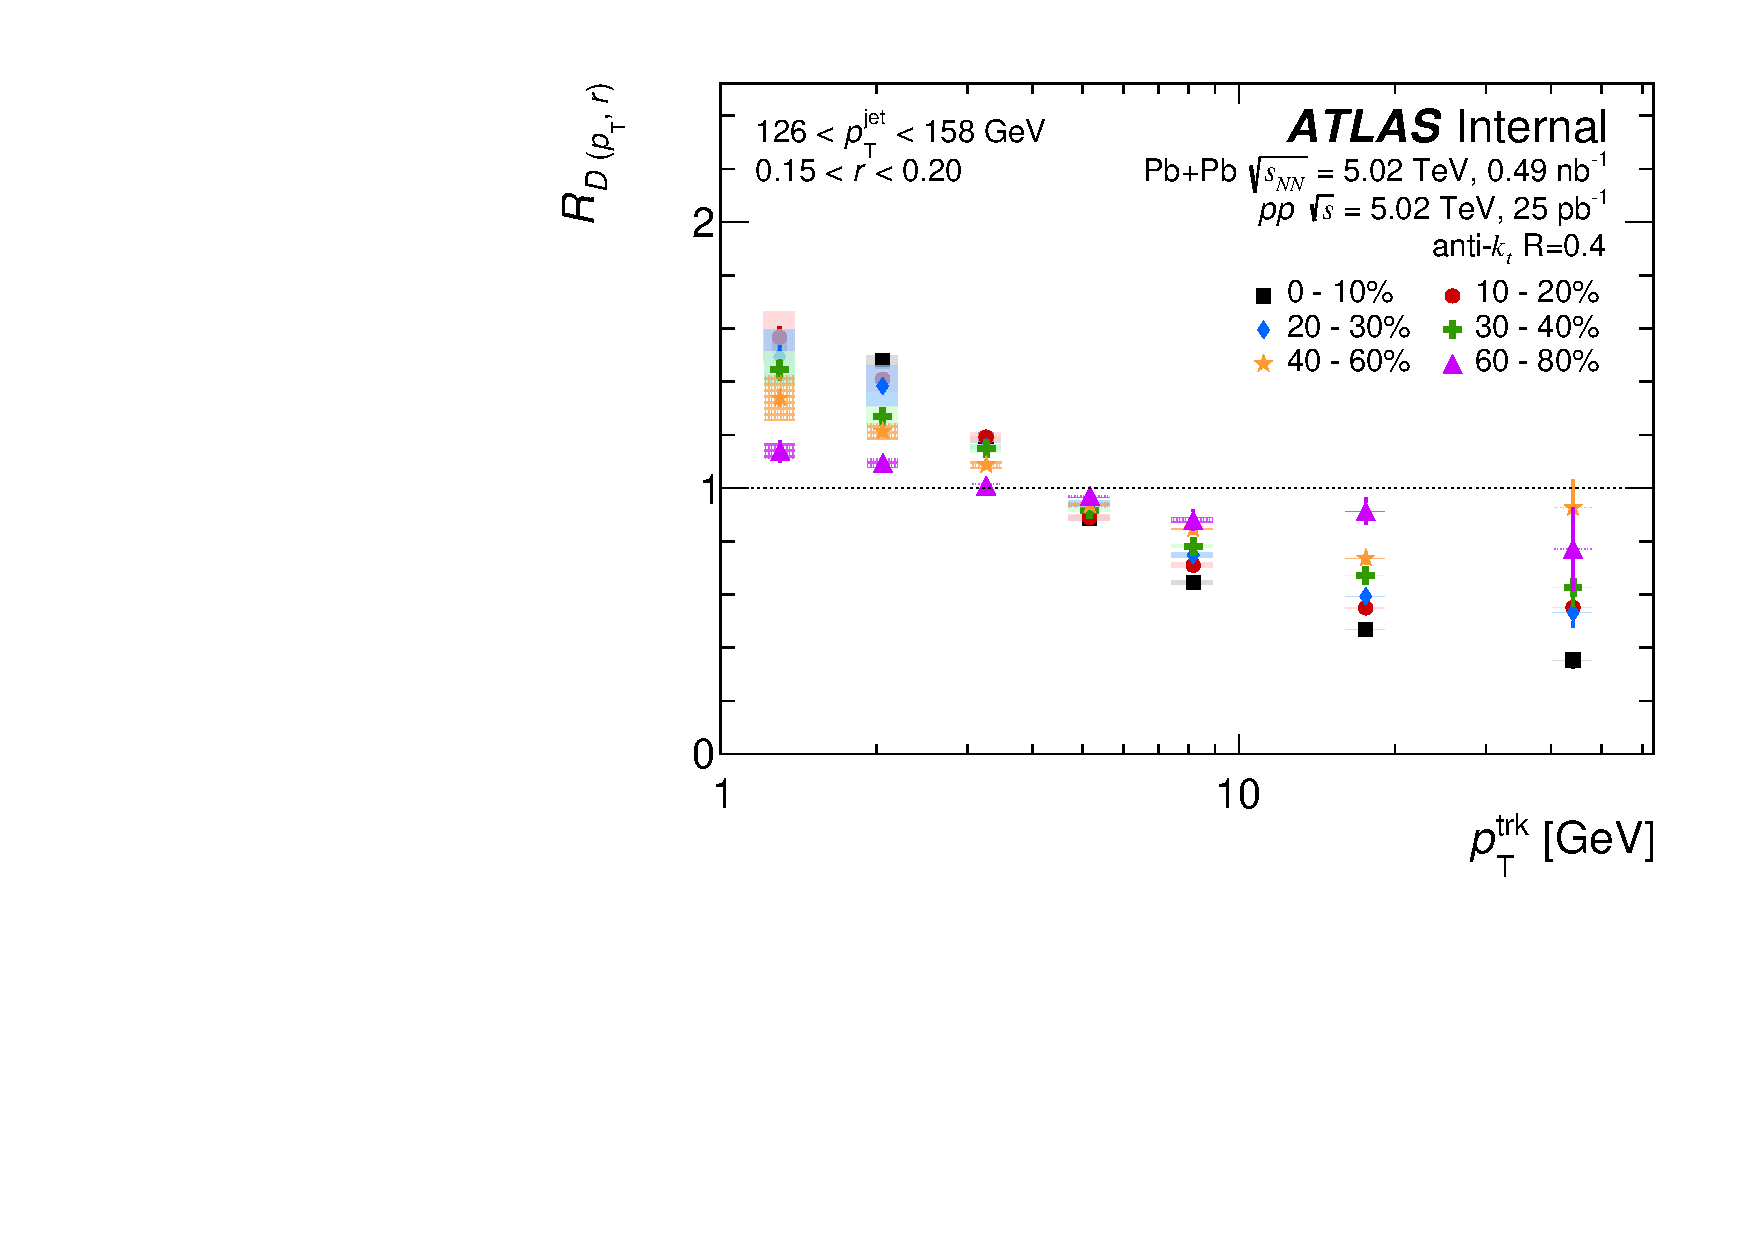
\includegraphics[width=0.5\textwidth]{results/RDpT_trkpt_jet7_dR3} &
%	 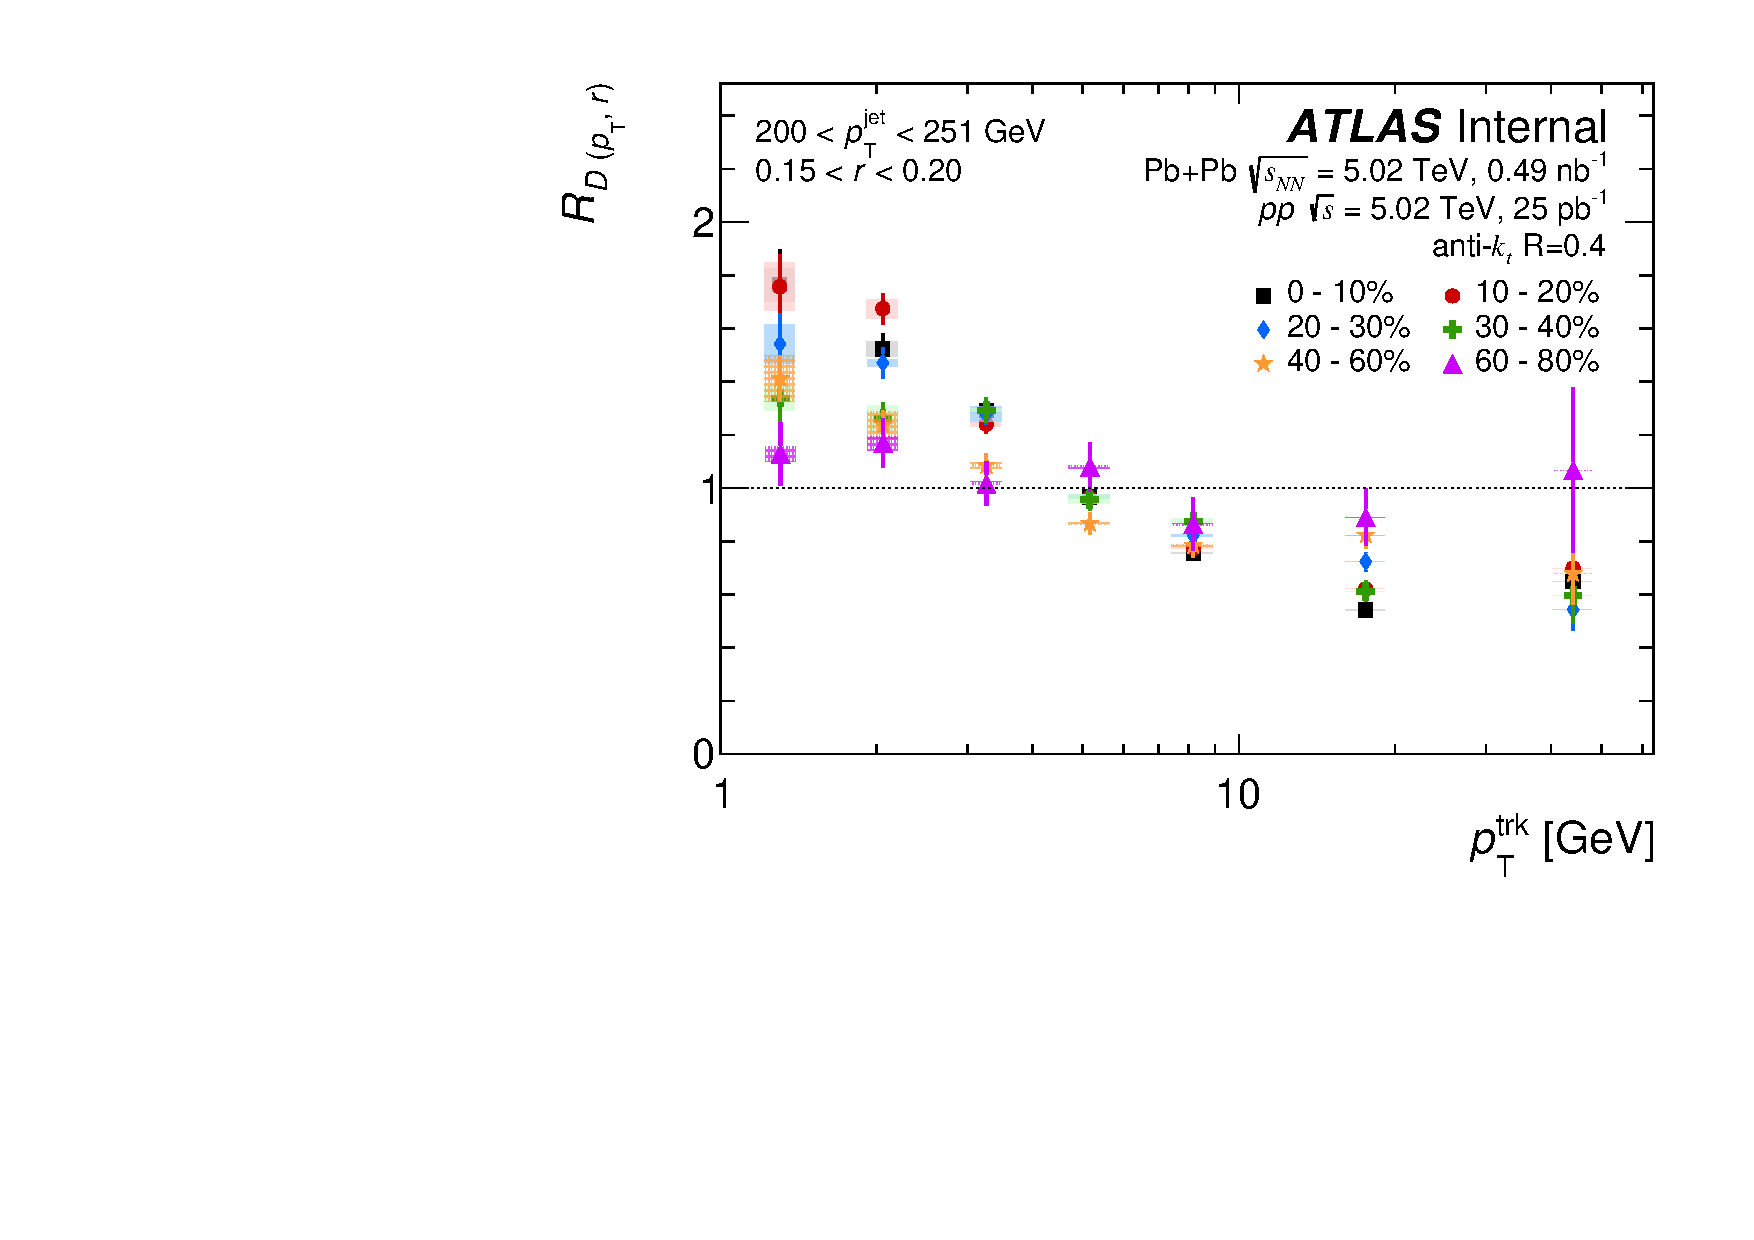
\includegraphics[width=0.5\textwidth]{results/RDpT_trkpt_jet9_dR3} \\
%	 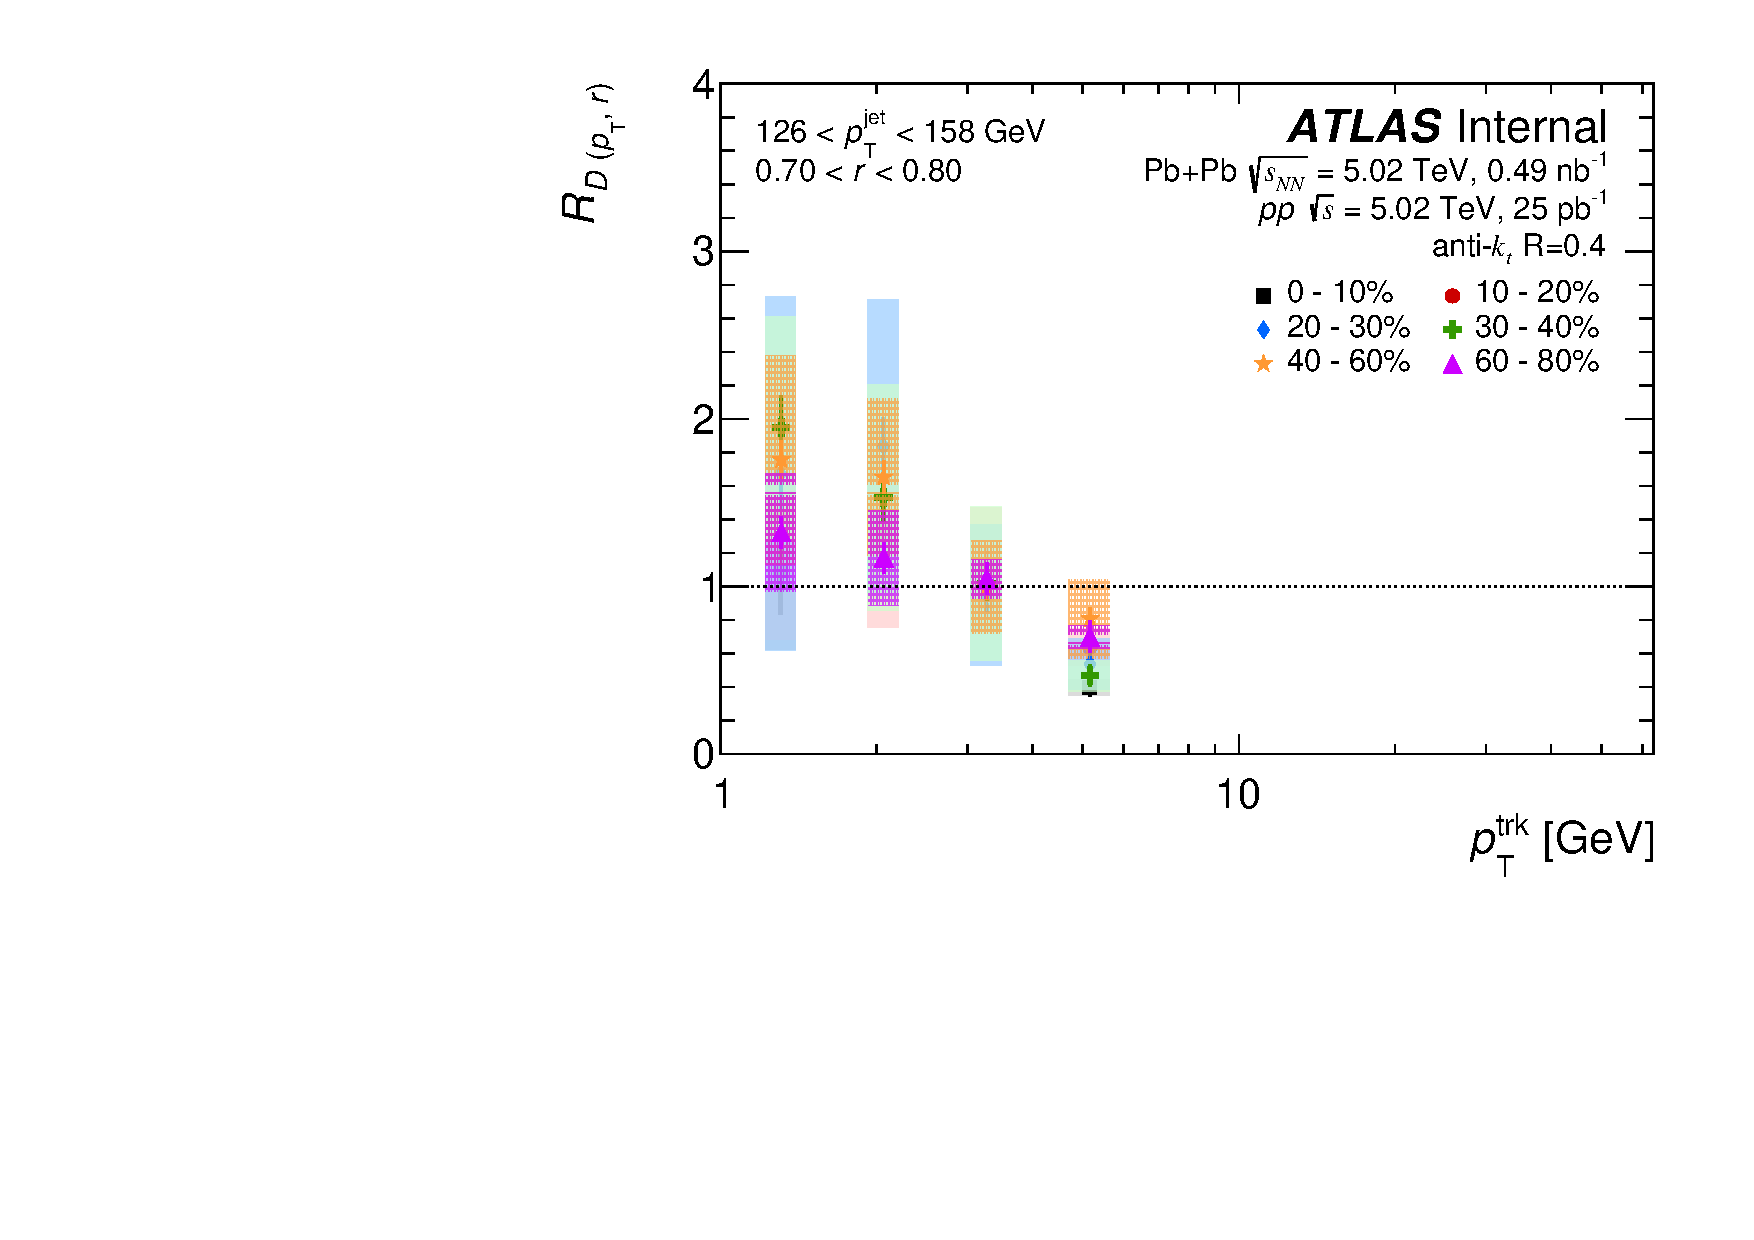
\includegraphics[width=0.5\textwidth]{results/RDpT_trkpt_jet7_dR10} &
%	 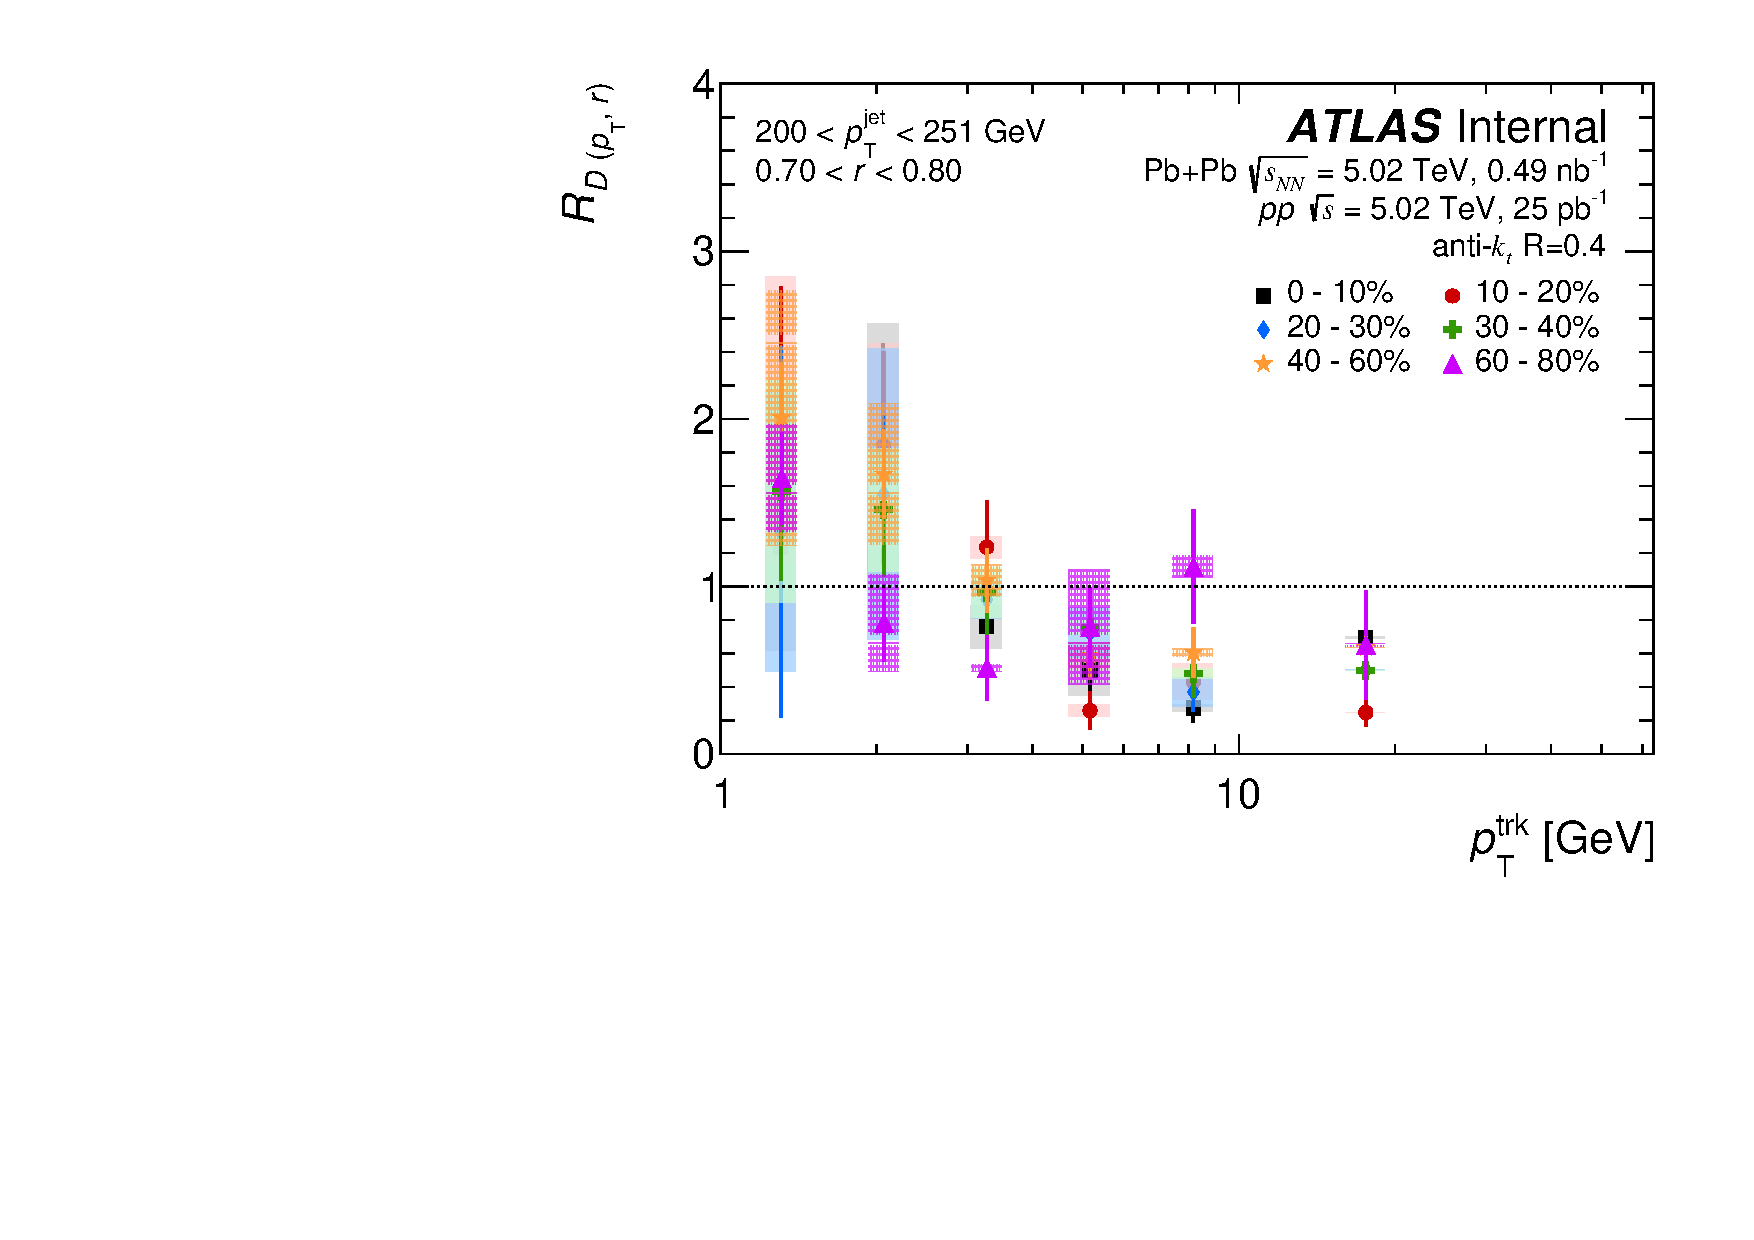
\includegraphics[width=0.5\textwidth]{results/RDpT_trkpt_jet9_dR10} \\
\end{tabular} }
   \caption{\RDptr\ for central \pbpb\ collisions as a function of \pt\ for different jet selections. The different colors represent different centrality bins. The vertical bars on the data points indicate statistical uncertainties while the shaded boxes indicate systematic uncertainties. The widths of the boxes are not indicative of the bin size and the points are shifted horizontally for better visibility.}
      \label{fig:rdptr_trk_cent}
\end{figure}
%%%%%%%%%%%%%




%% DeltaDpT
Differences between the \Dptr\ distributions in \pbpb\ and \pp, given as:

\begin{align}
\DeltaDptr = \Dptr_{\mathrm{Pb+Pb}} - \Dptr_{pp}
\end{align}

are presented as a function of $r$ for different \pt\ selections in 0--10\% central collisions in Figure~\ref{fig:deltadptr}. 
These distributions show an excess  in the charged-particle yield density for \pbpb\ collisions compared to \pp\ collisions for charged particles with $\pt <$~4.0\GeV. This excess ranges from 0.5 to 4 particles per unit area at 1 \GeV\ in 126--158~\GeV\ jets for 0--10\% central \pbpb\ collisions and increases with increasing \ptjet. 
A depletion for highe \pt\ particles is at most 0.5 particles per unit area for 126--158~\GeV\ jets in  0--10\% central \pbpb\ collisions and increases for higher \ptjet. 
For particles with 25.1~$< \pt <$~63.1~\GeV, the \DeltaDptr\ distribution is consistent with unity over the entire 
measured range of \rvar\ and \ptjet.
There is a minimum in the \DeltaDptr distribution for charged particles with \mbox{$ 4.0 < \pt <  25.1$}~\GeV\ at $0.05 < \rvar < 0.10$ that is seen at all \ptjet\ ranges under investigation.

\begin{figure}
\centering{
\begin{tabular}{cc}
	 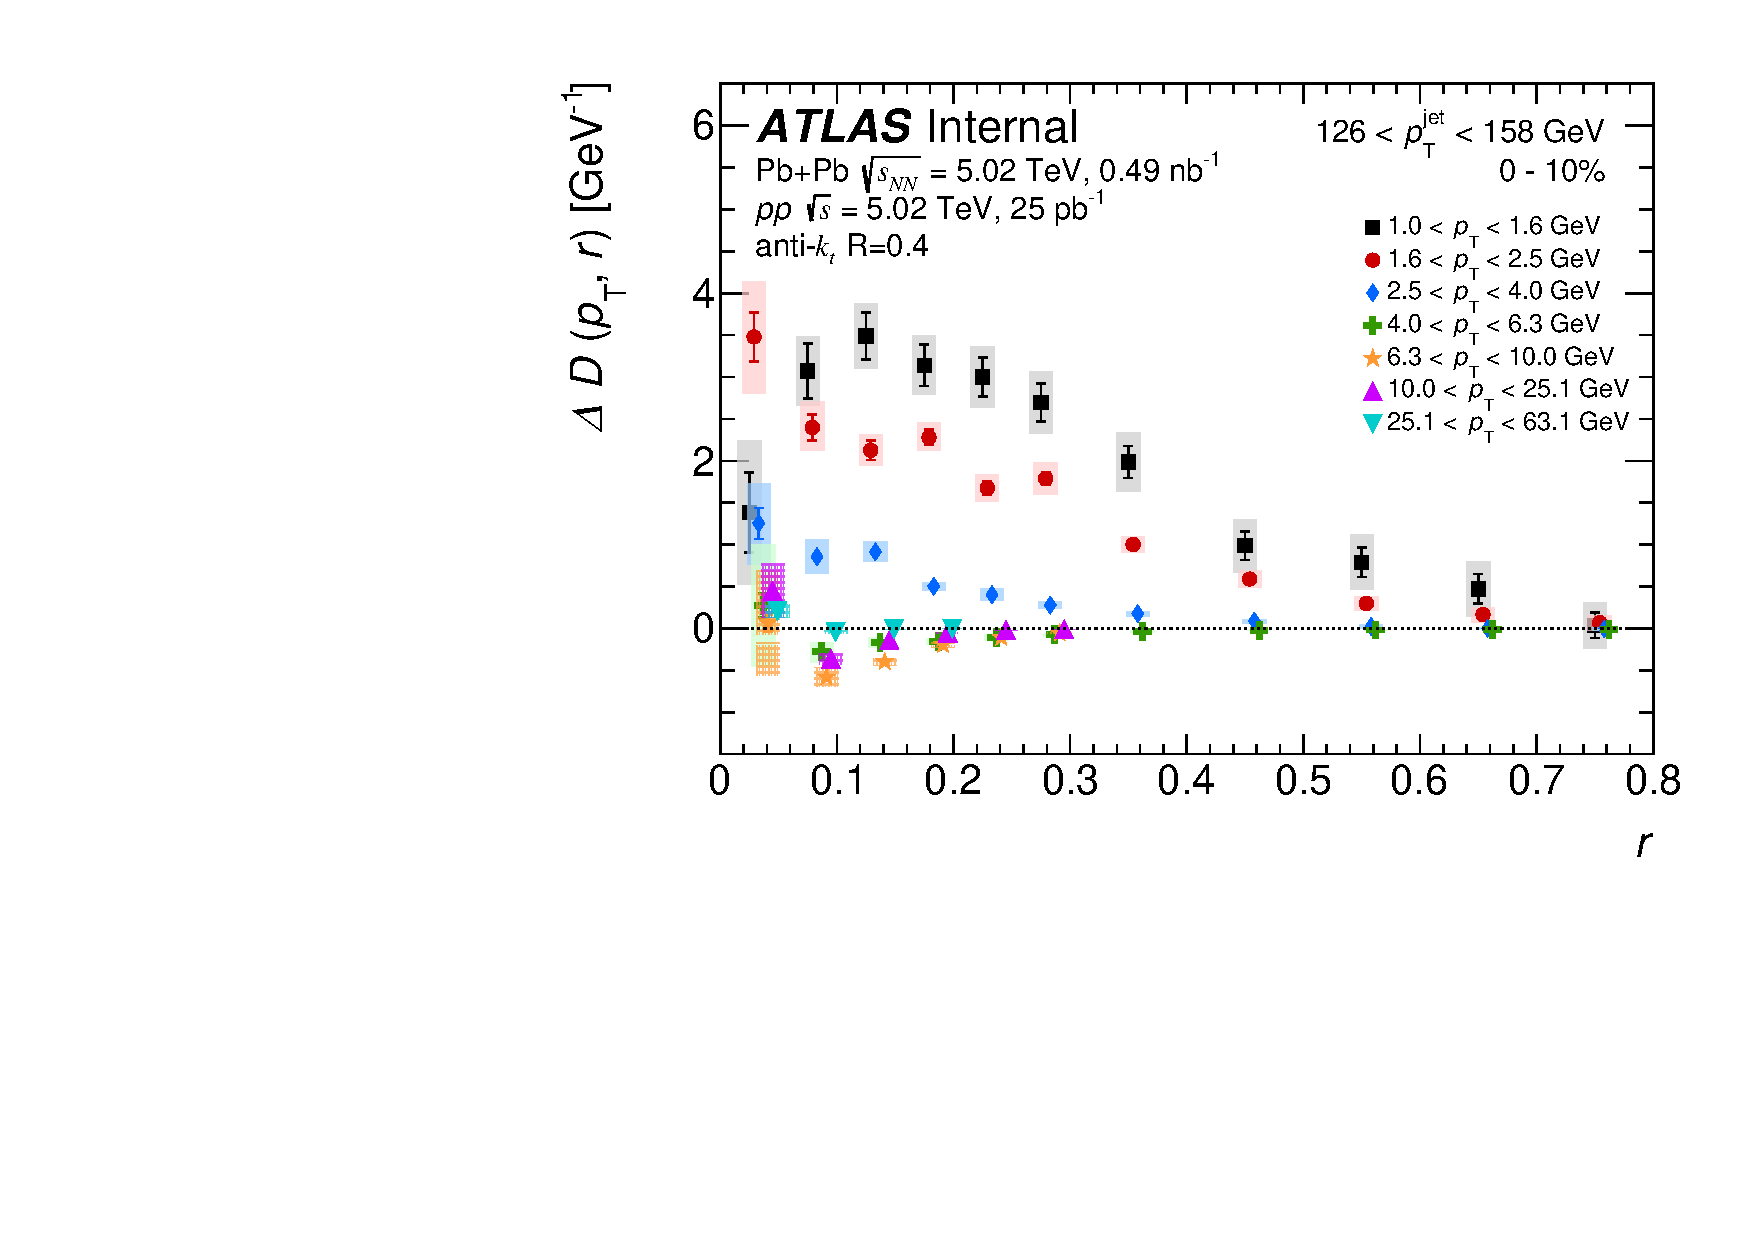
\includegraphics[width=0.5\textwidth]{results/DeltaDpT_dR_jet7_cent0} &
	 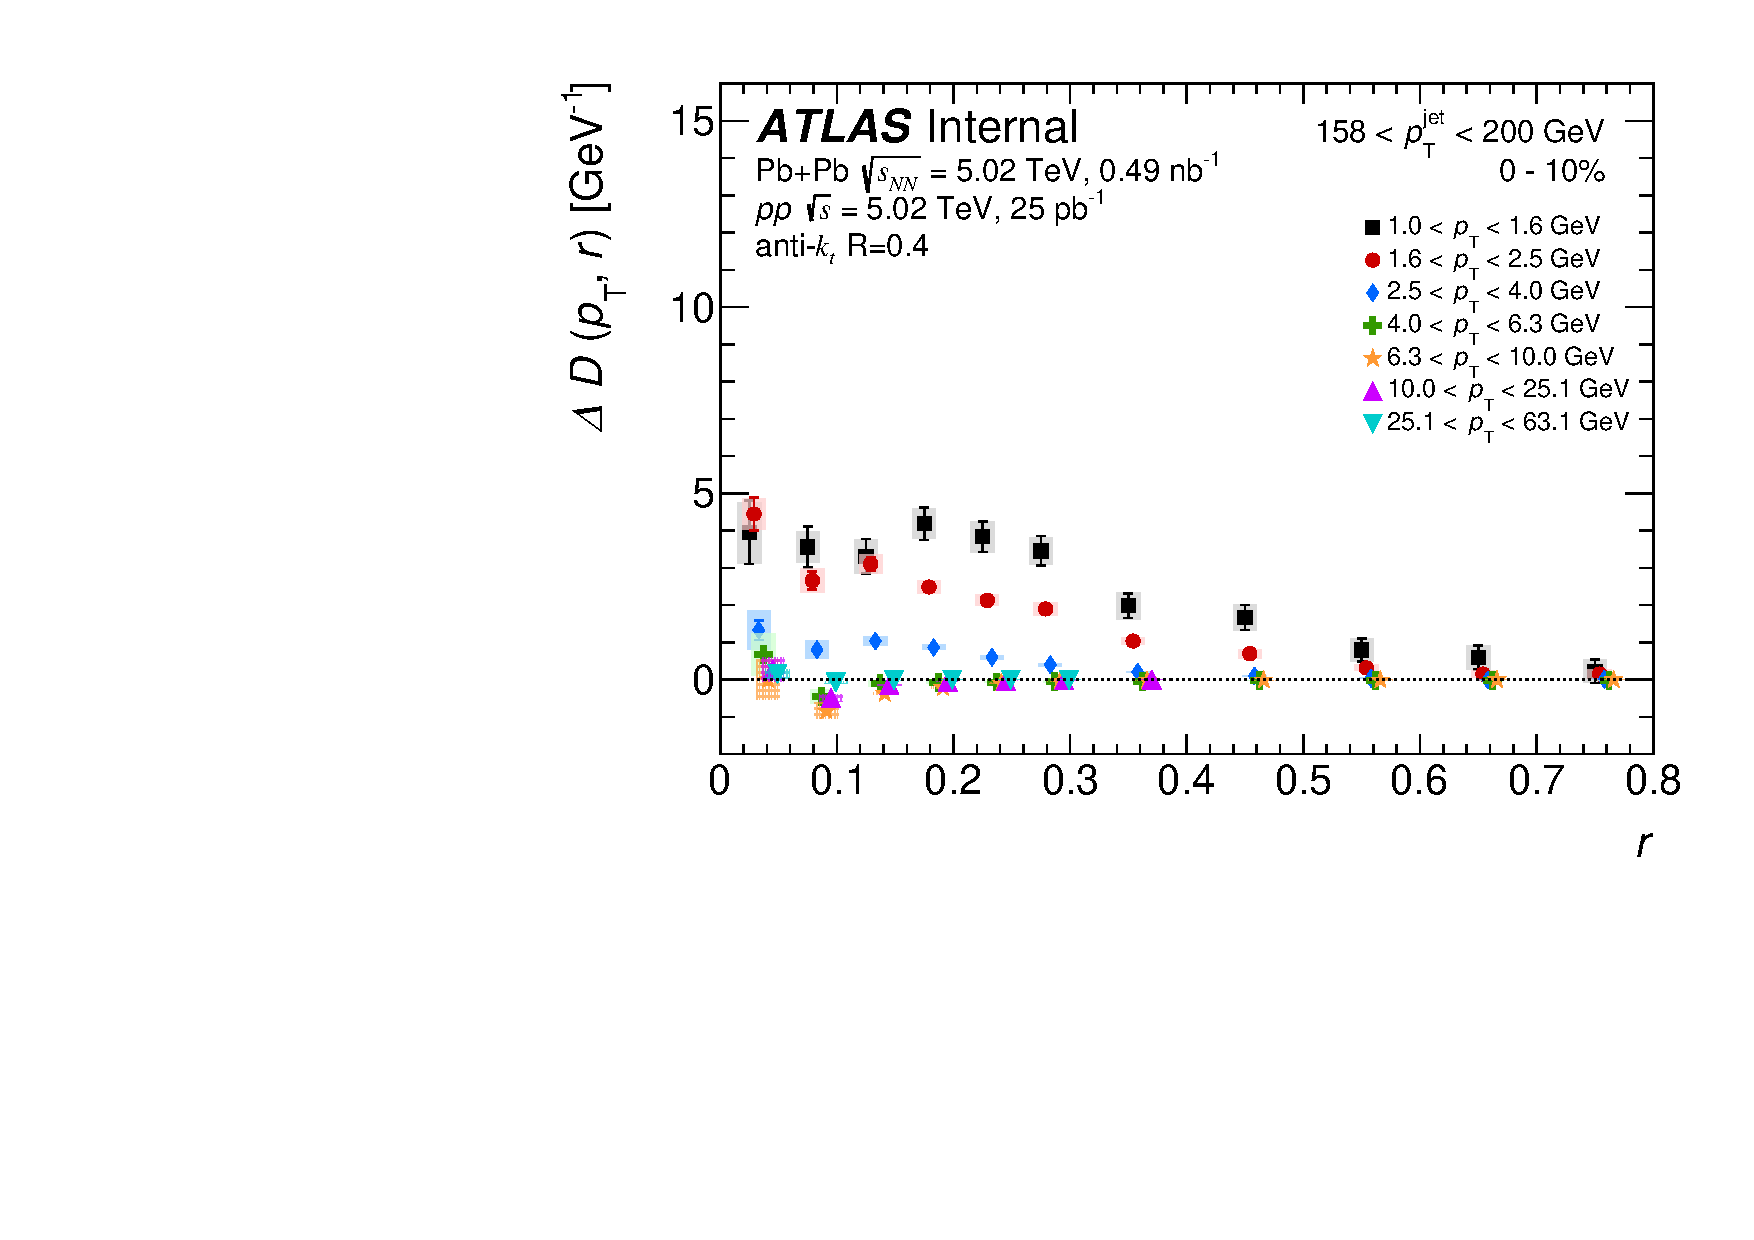
\includegraphics[width=0.5\textwidth]{results/DeltaDpT_dR_jet8_cent0} \\
	 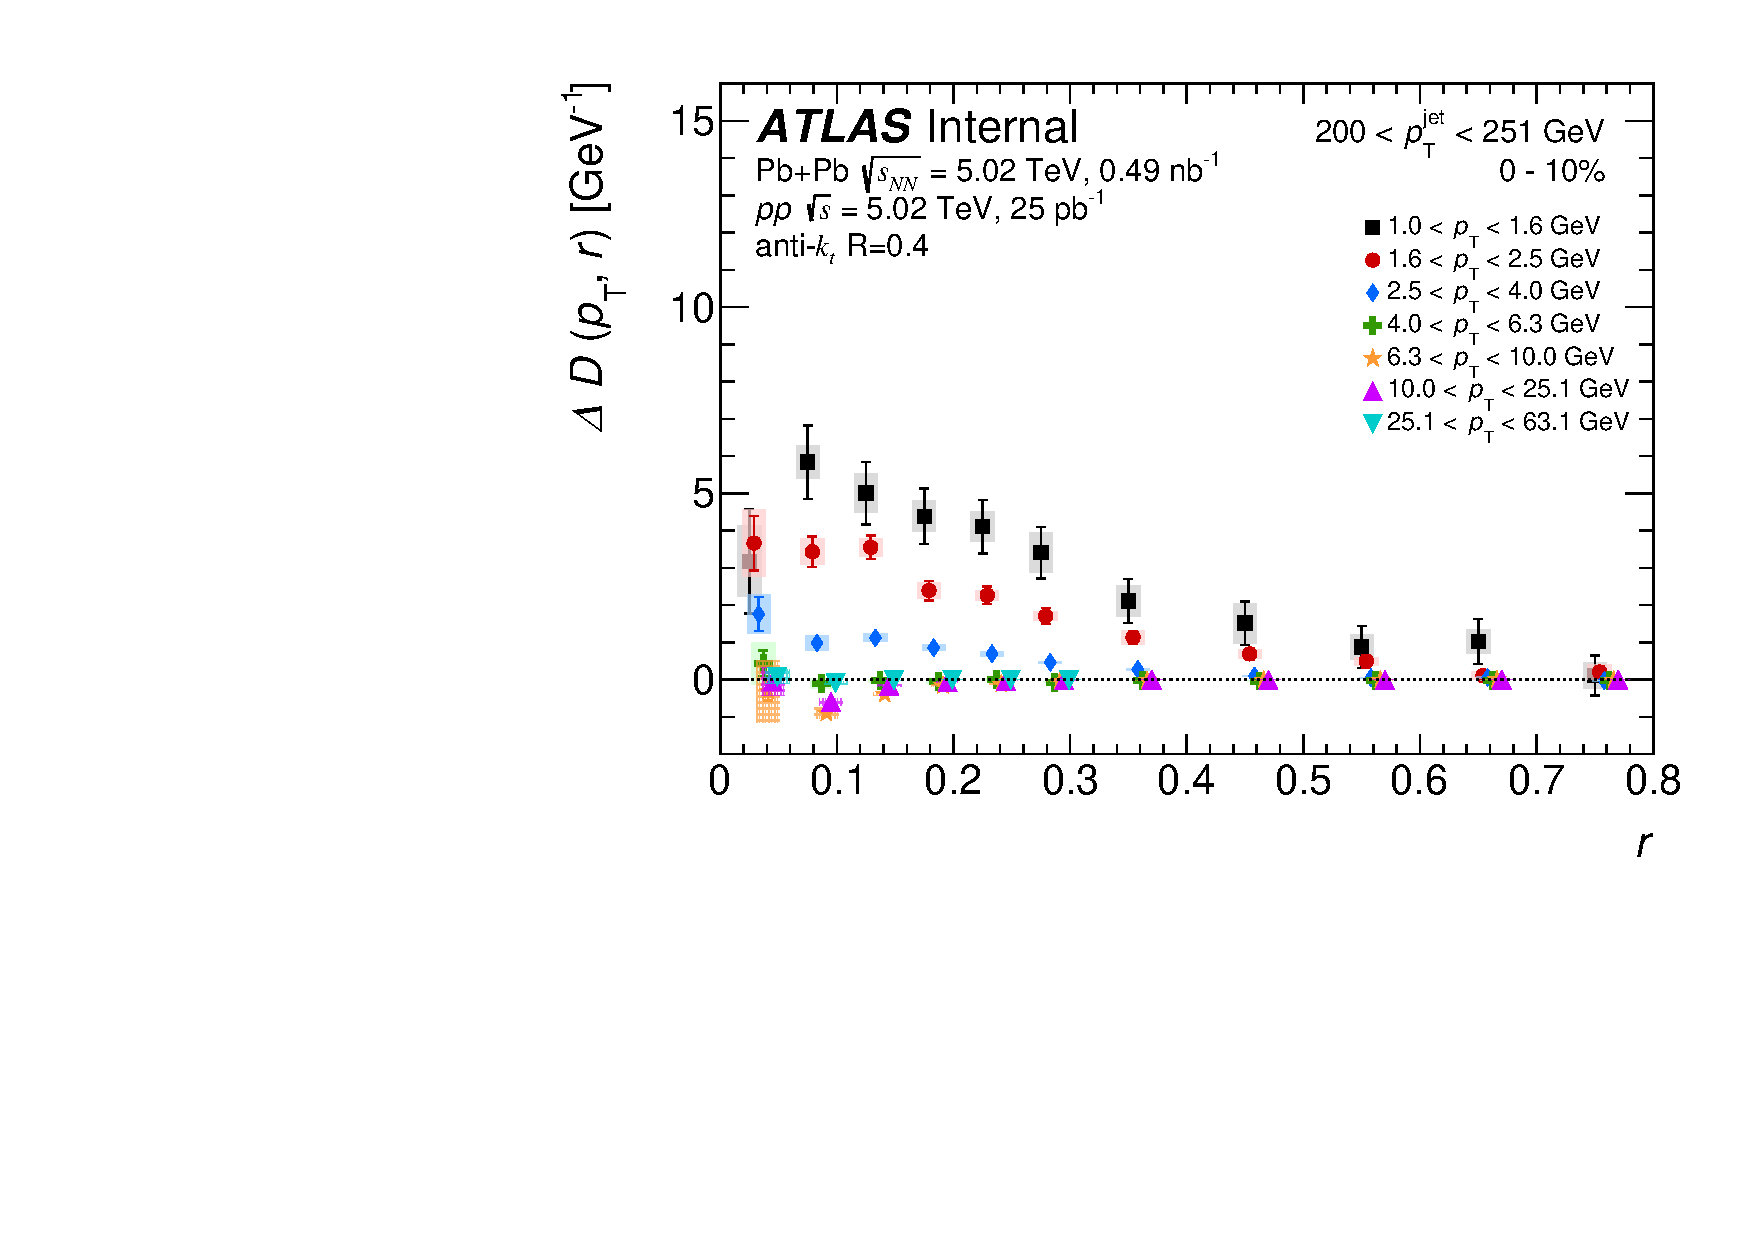
\includegraphics[width=0.5\textwidth]{results/DeltaDpT_dR_jet9_cent0} &
	 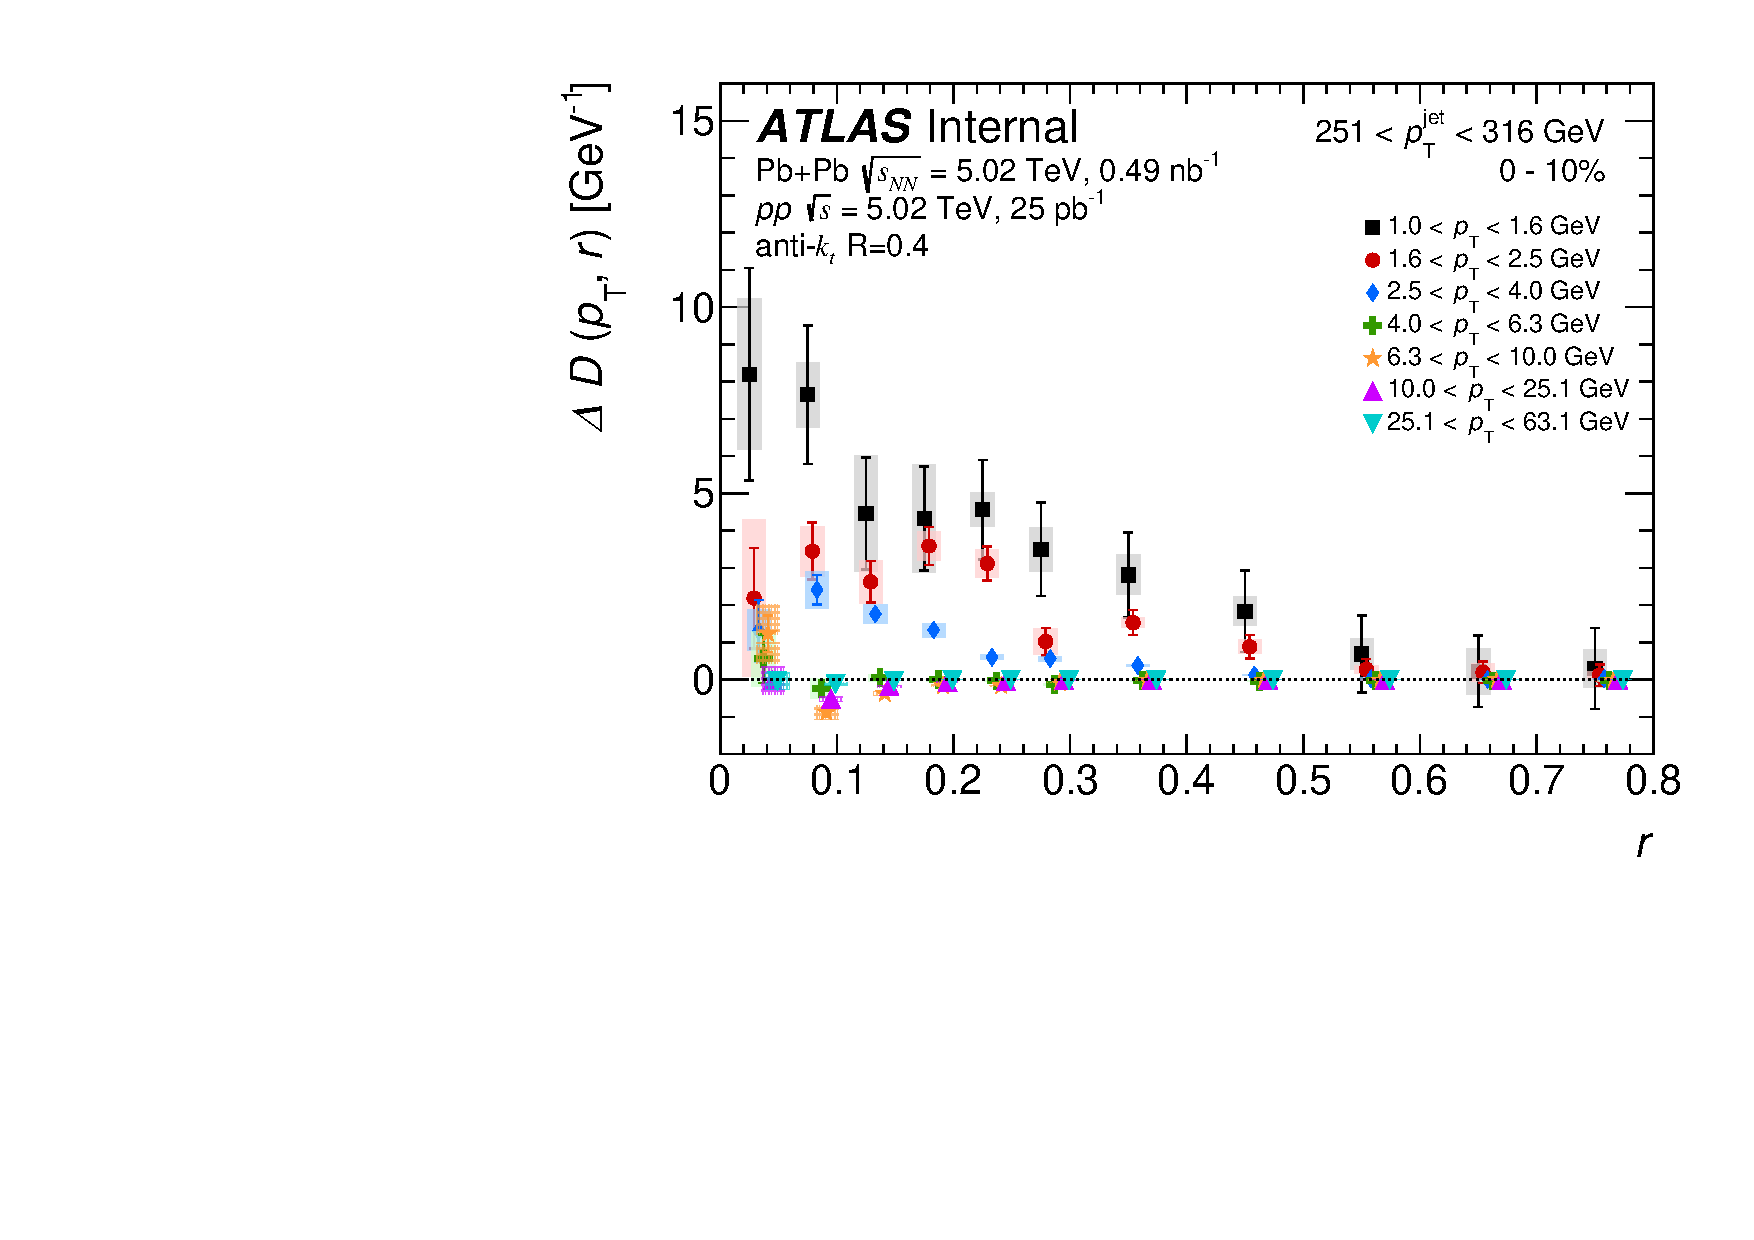
\includegraphics[width=0.5\textwidth]{results/DeltaDpT_dR_jet10_cent0} \\
\end{tabular} }
   \caption{\DeltaDptr\ as a function of \rvar\ in central collisions for all \pt\ ranges in four \ptjet\ selections: 126--158~\GeV, 158--200~\GeV, 200--251~\GeV, and 251--316~\GeV. The vertical bars on the data points indicate statistical uncertainties while the shaded boxes indicate systematic uncertainties. The widths of the boxes are not indicative of the bin size and the points are shifted horizontally for better visibility. }
      \label{fig:deltadptr}
\end{figure}
%%%%%%%%%%%%%

%\subparagraph{Integrated plots}
The \Dptr\ distribution can be integrated for particles with \pt\ < 4 GeV to construct the quantities $\Theta$ and $P$.
\begin{align}
   \Theta(\rvar)_{\mathrm{x}} &= \int_1^{4} \Dptr |_{\mathrm{x}} \fd \pt \\
   P(\rvar)_{\mathrm{x}} &= \int_0^r \int_1^{4} \Dptr \fd \pt \fd r' |_{\mathrm{x}}
\end{align}
where x $\in [\pp, \pbpb]$. These can be compared between the \pp\ and \pbpb\ systems to give the following distributions:
\begin{align}
 \Delta_\Theta(\rvar) = \Theta(\rvar)_{\mathrm{Pb+Pb}} - \Theta(\rvar)_{pp} & \qquad \Delta_P(\rvar) = P(\rvar)_{\mathrm{Pb+Pb}} - P(\rvar)_{pp} \\
   R_\Theta(\rvar) = \frac{\Theta(\rvar){\mathrm{Pb+Pb}}}{\Theta(\rvar)_{\mathrm{pp}}} &  \qquad R_{P(\rvar)} = \frac{P(\rvar)_{\mathrm{Pb+Pb}}}{P(\rvar)_{pp}}
\end{align}
These variables provide aggregate information for particles with \pt < 4 GeV, both differentially and cumulatively in \rvar.
Figure~\ref{fig:deltaPdeltaT} shows the \DeltaTheta\ and \DeltaP\ distributions as a function of \rvar. The \ptjet\ dependence to the excess in charged-particle density can be seen clearly. Moreover, the \DeltaP\ distribution shows that there is an extra particle density of 0.5 when integrated up to $\rvar = 0.8$ around the jet cone. Figure~\ref{fig:RPRT} shows the \RTheta\ and \RP\ distributions as a function of \rvar. It can be seen that the size of the enhancement is approximately constant for $r > 0.5$.

%\begin{align}
%\Delta_\Theta = \int_1^{4} \Dpt_{\mathrm{PbPb}} - \Dpt_{\mathrm{pp}} \fd \pt
%\end{align}
\begin{figure}
\centering{
\begin{tabular}{cc}
	 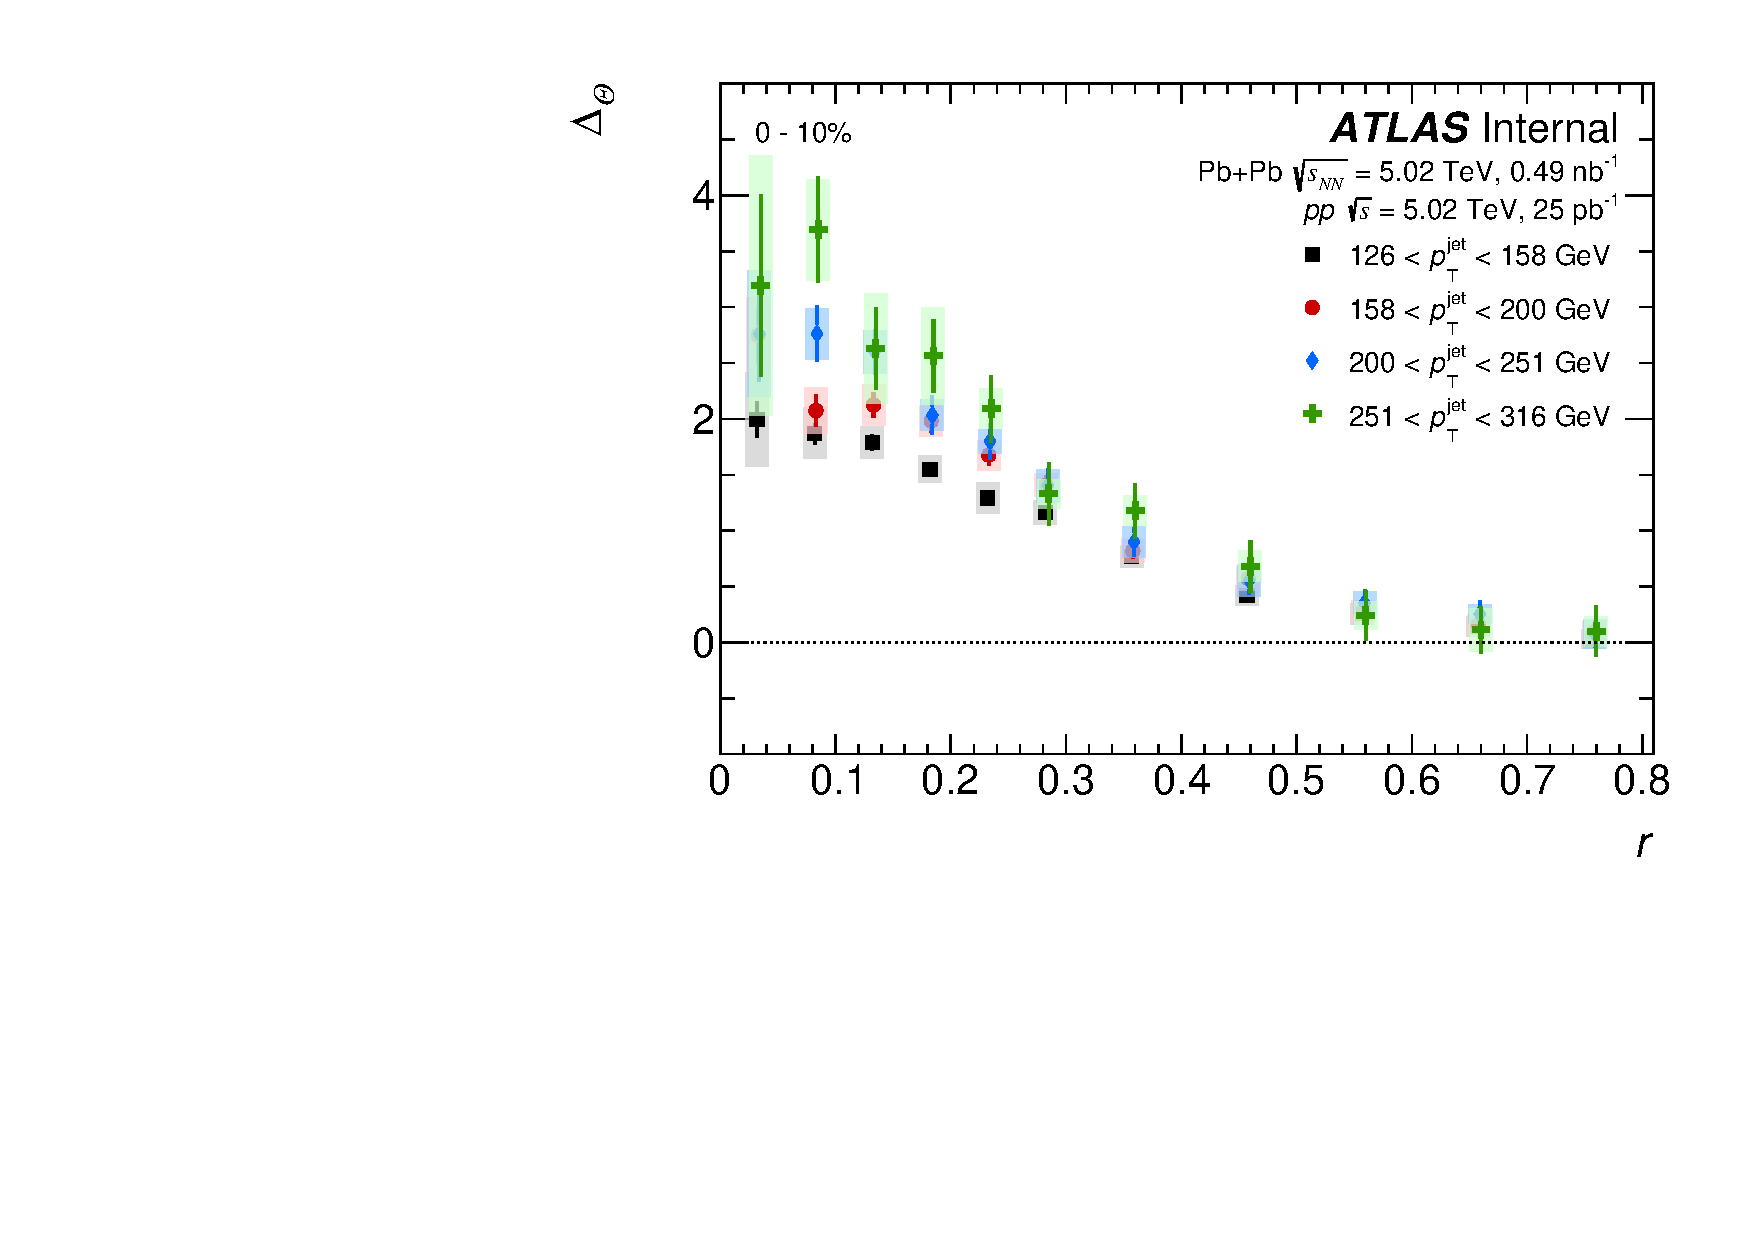
\includegraphics[width=0.5\textwidth]{results/DeltaDpT_lowpt_integ_cent0.pdf} &
	 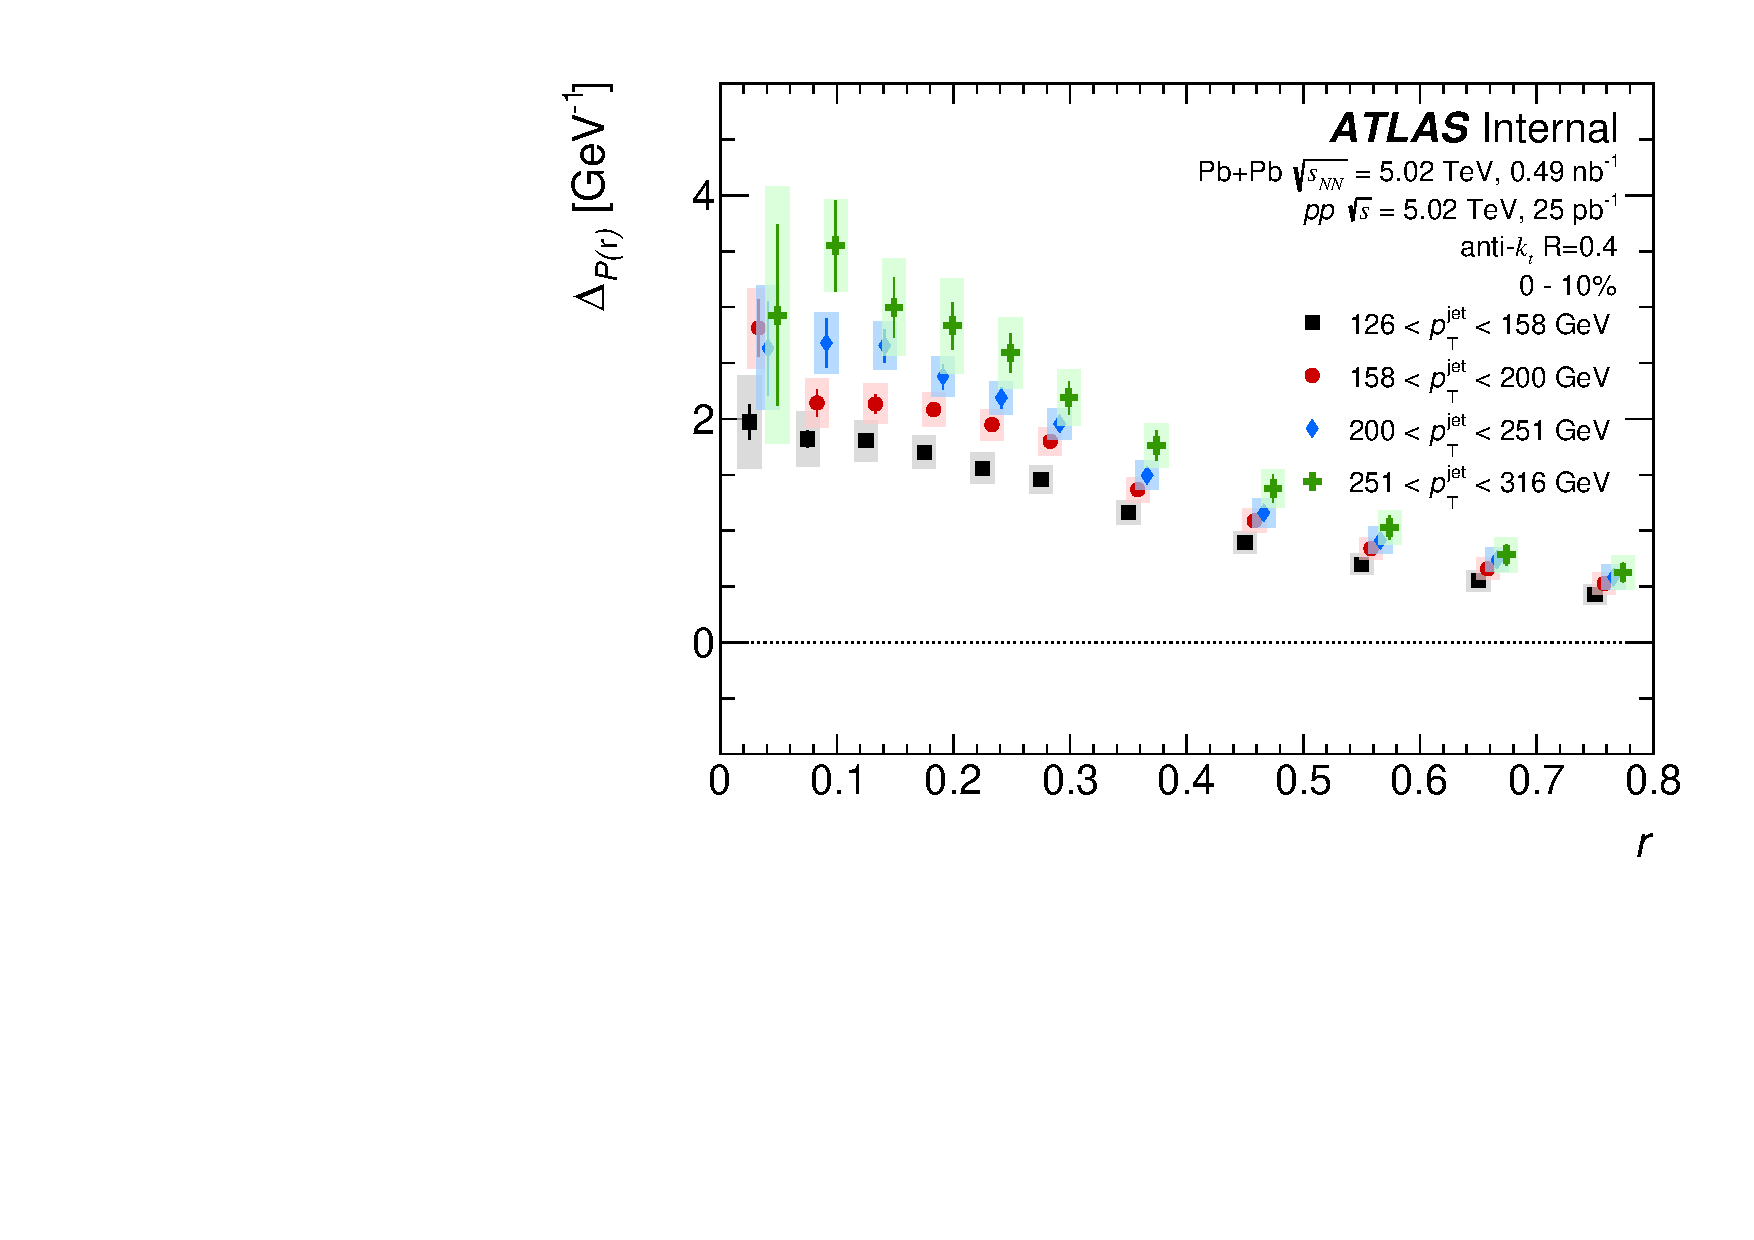
\includegraphics[width=0.5\textwidth]{results/DeltaDpT_jetshape_cent0.pdf} \\
\end{tabular} }
   \caption{\DeltaTheta\ (left) and \DeltaP\ (right) as a function of \rvar\ in central collisions for charged-particles with \pt\ < 4 GeV ranges in four \ptjet\ selections: 126--158~\GeV, 158--200~\GeV, 200--251~\GeV, and 251--316~\GeV. The vertical bars on the data points indicate statistical uncertainties while the shaded boxes indicate systematic uncertainties. The widths of the boxes are not indicative of the bin size and the points are shifted horizontally for better visibility. }
      \label{fig:deltaPdeltaT}
\end{figure}


\begin{figure}
\centering{
\begin{tabular}{cc}
	 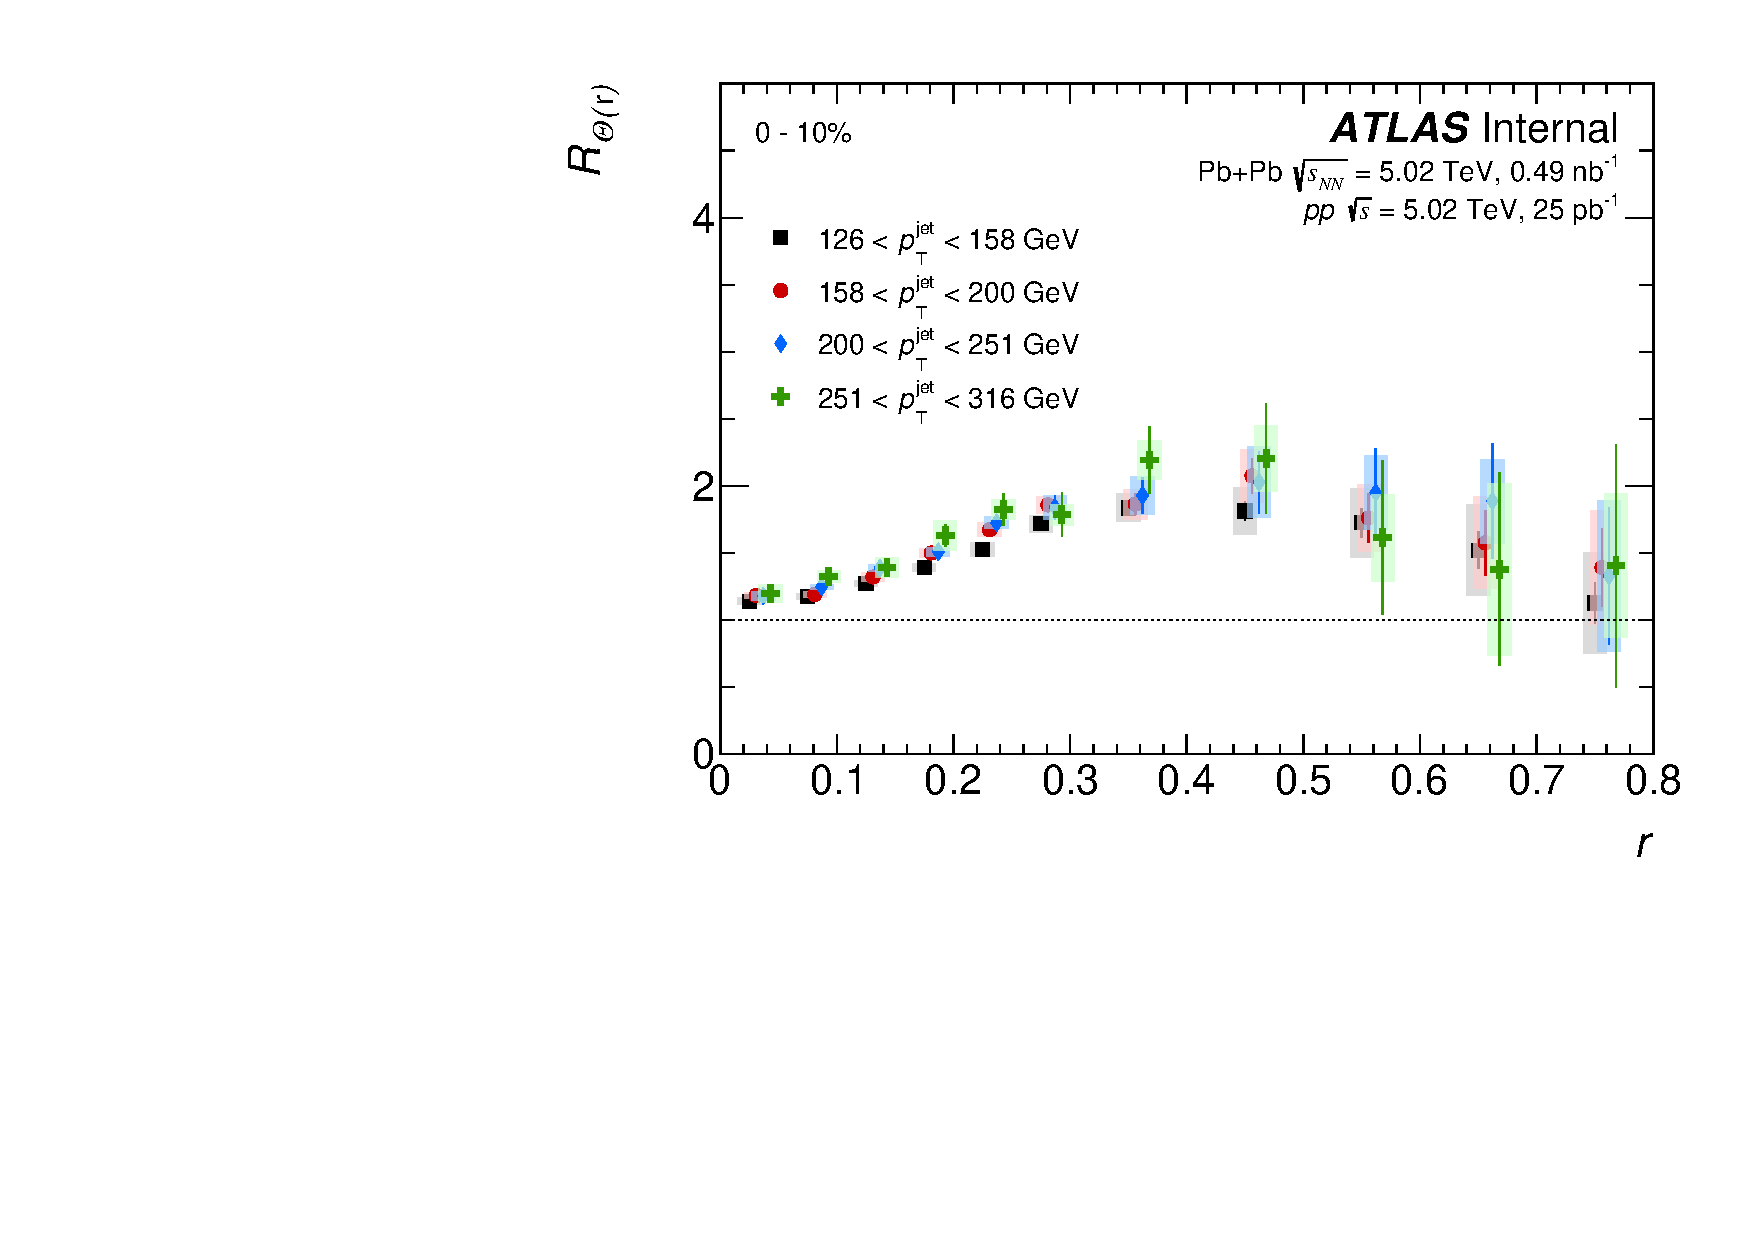
\includegraphics[width=0.5\textwidth]{results/RDpT_lowpt_integ_cent0.pdf} &
	 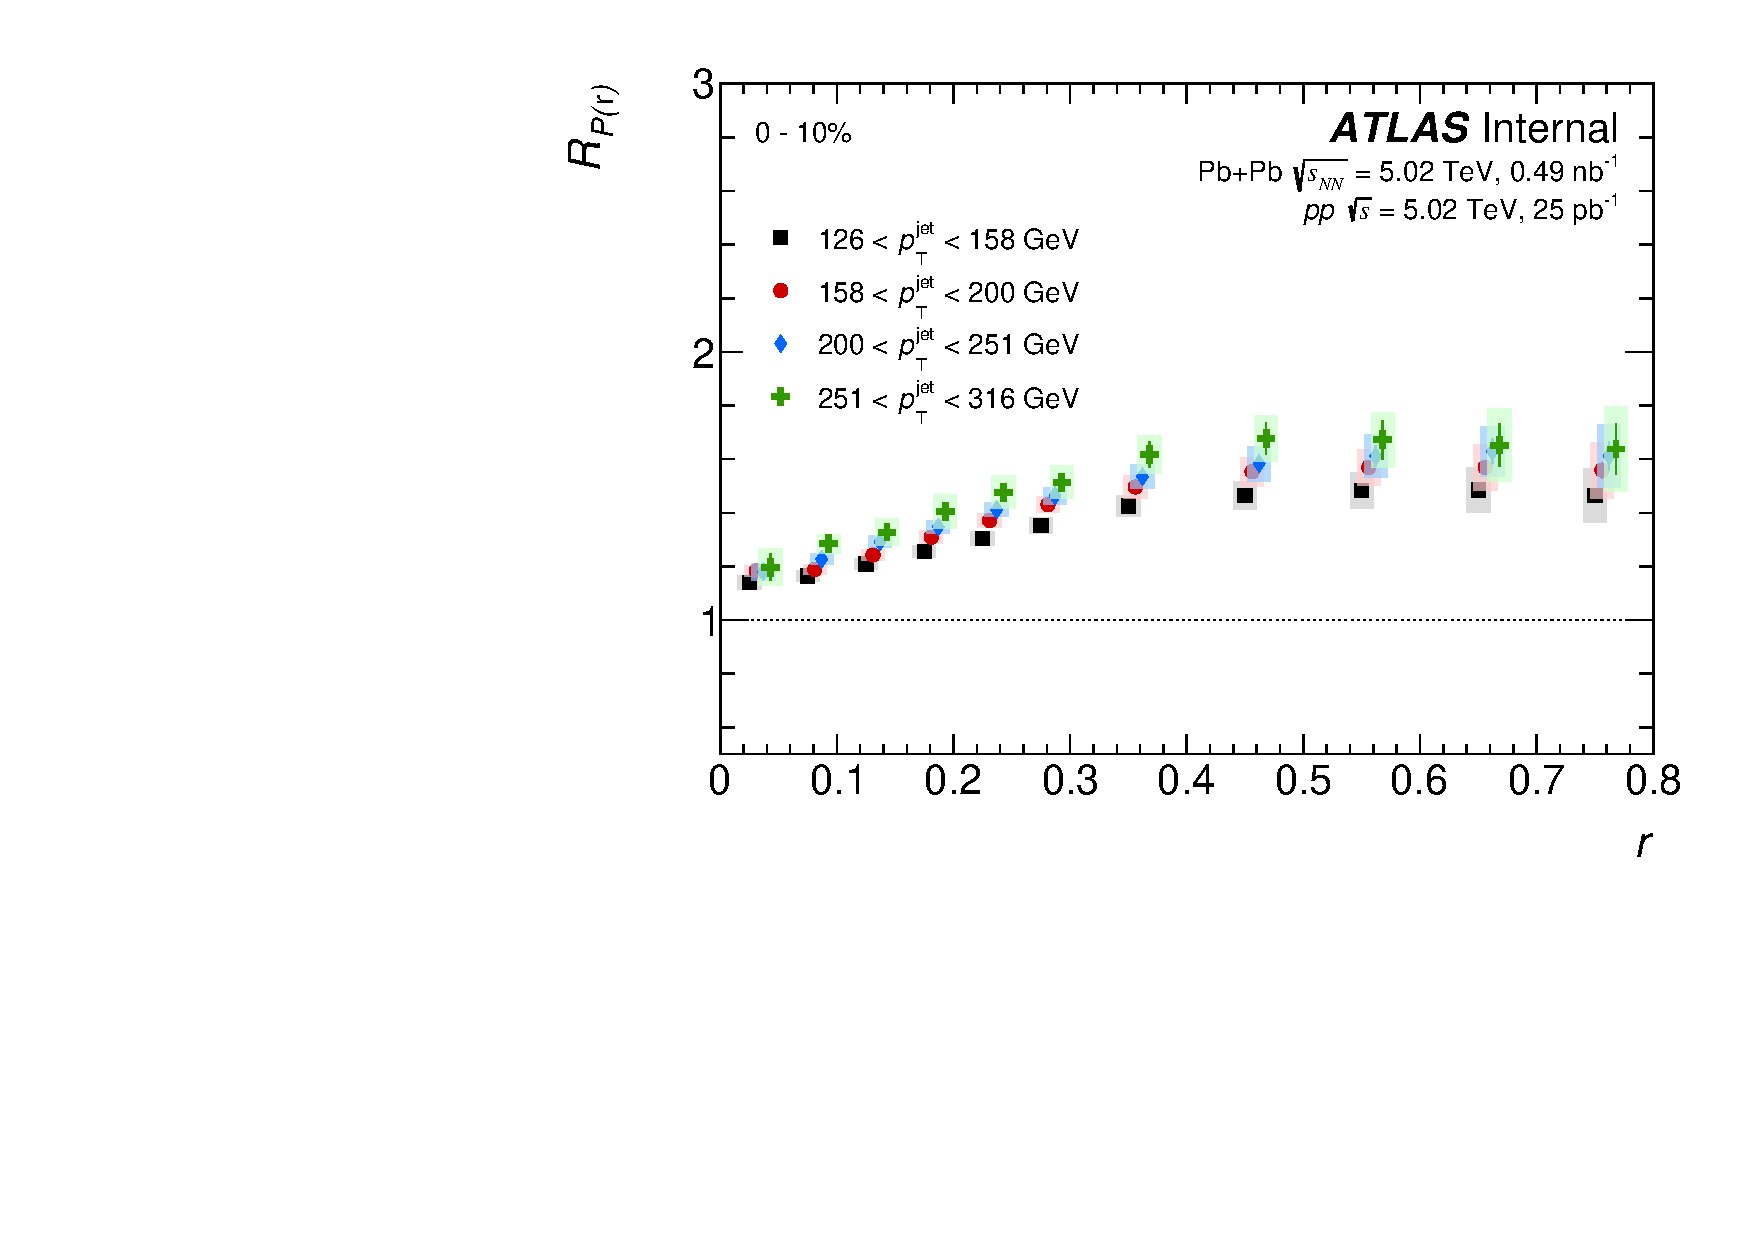
\includegraphics[width=0.5\textwidth]{results/RDpT_jetshape_cent0.pdf} \\
\end{tabular} }
   \caption{\RTheta\ (left) and \RP\ (right) as a function of \rvar\ in central collisions for charged-particles with \pt\ < 4 GeV ranges in four \ptjet\ selections: 126--158~\GeV, 158--200~\GeV, 200--251~\GeV, and 251--316~\GeV. The vertical bars on the data points indicate statistical uncertainties while the shaded boxes indicate systematic uncertainties. The widths of the boxes are not indicative of the bin size and the points are shifted horizontally for better visibility. }
      \label{fig:RPRT}
\end{figure}



%
%%% RDpT as function of jet pT
%\begin{figure}
%\centering{
%\begin{tabular}{cc}
%	 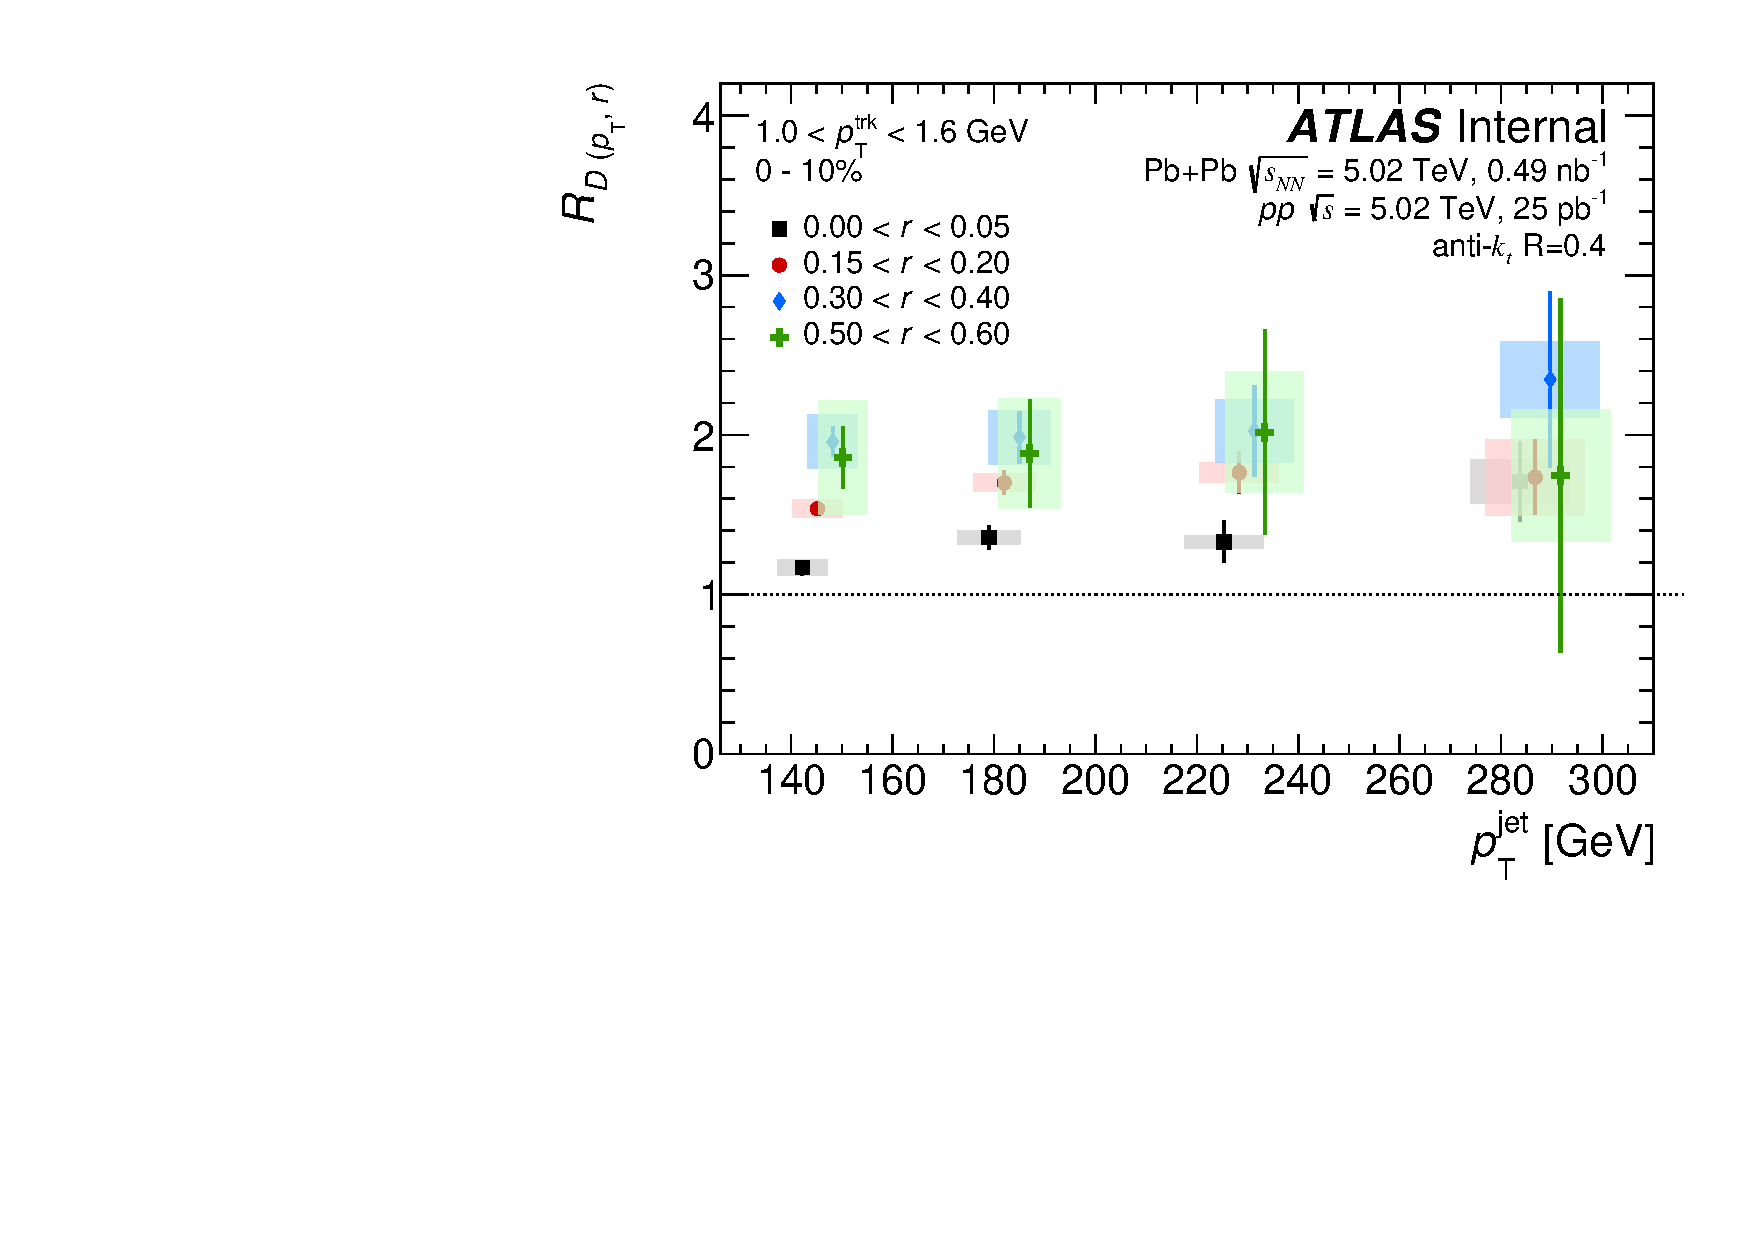
\includegraphics[width=0.45\textwidth]{results/RDpT_jetpt_trk2_cent0} &
%	 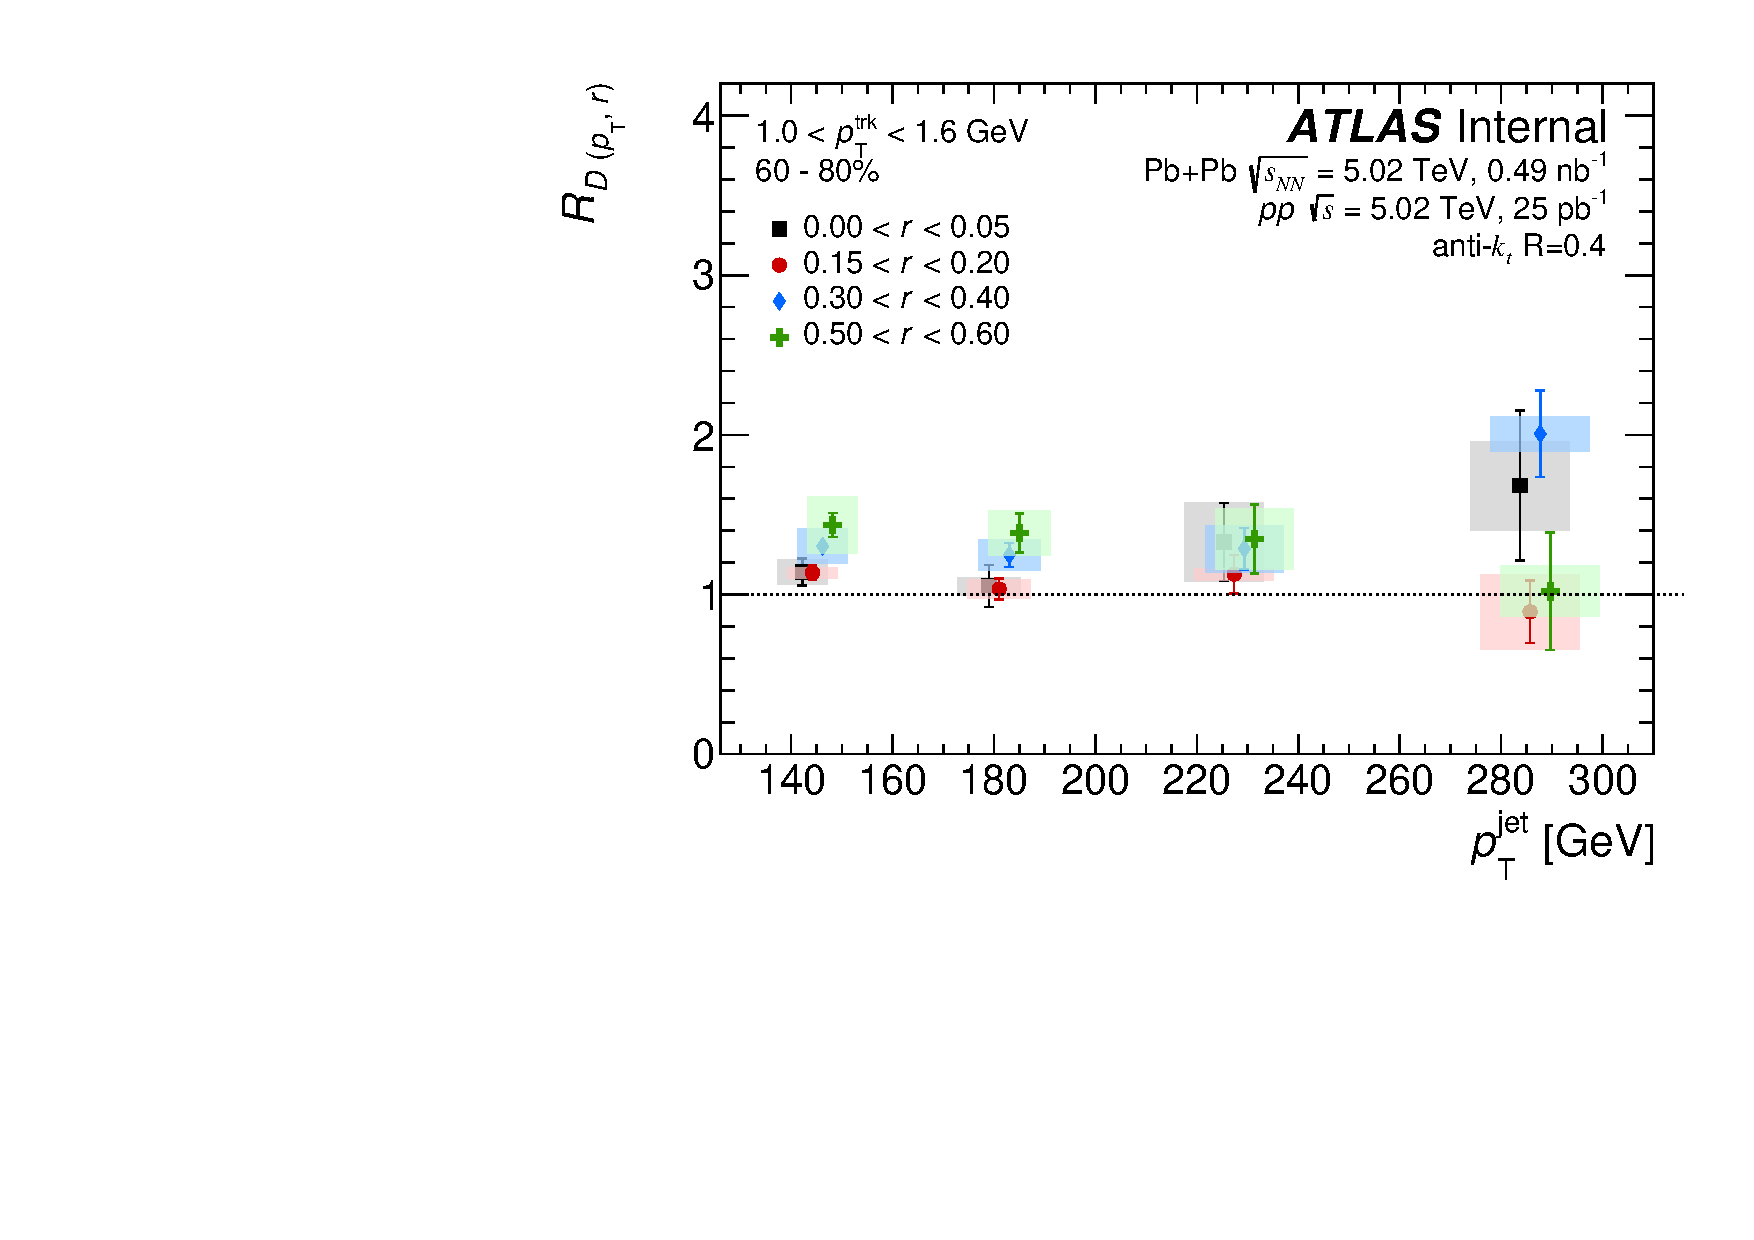
\includegraphics[width=0.45\textwidth]{results/RDpT_jetpt_trk2_cent5} \\
%	 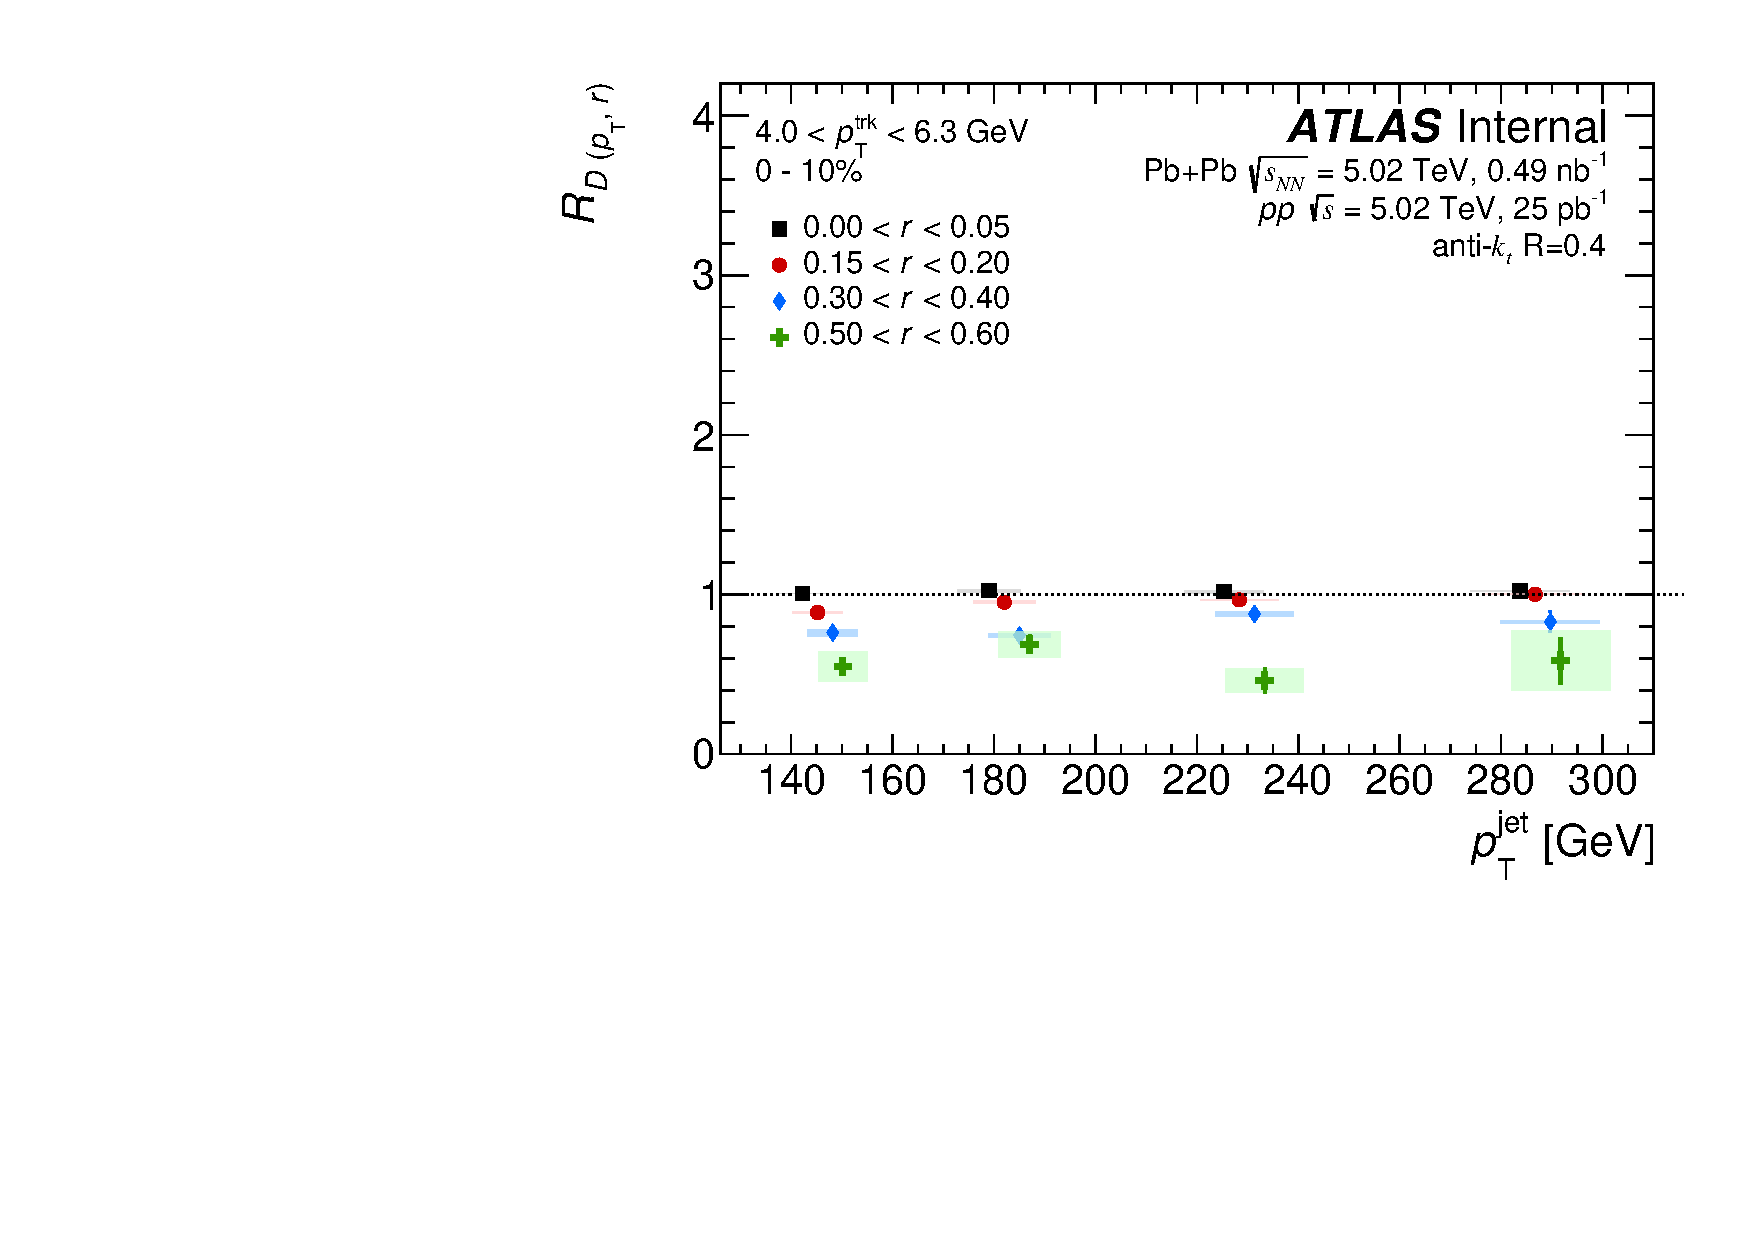
\includegraphics[width=0.45\textwidth]{results/RDpT_jetpt_trk5_cent0} &
%	 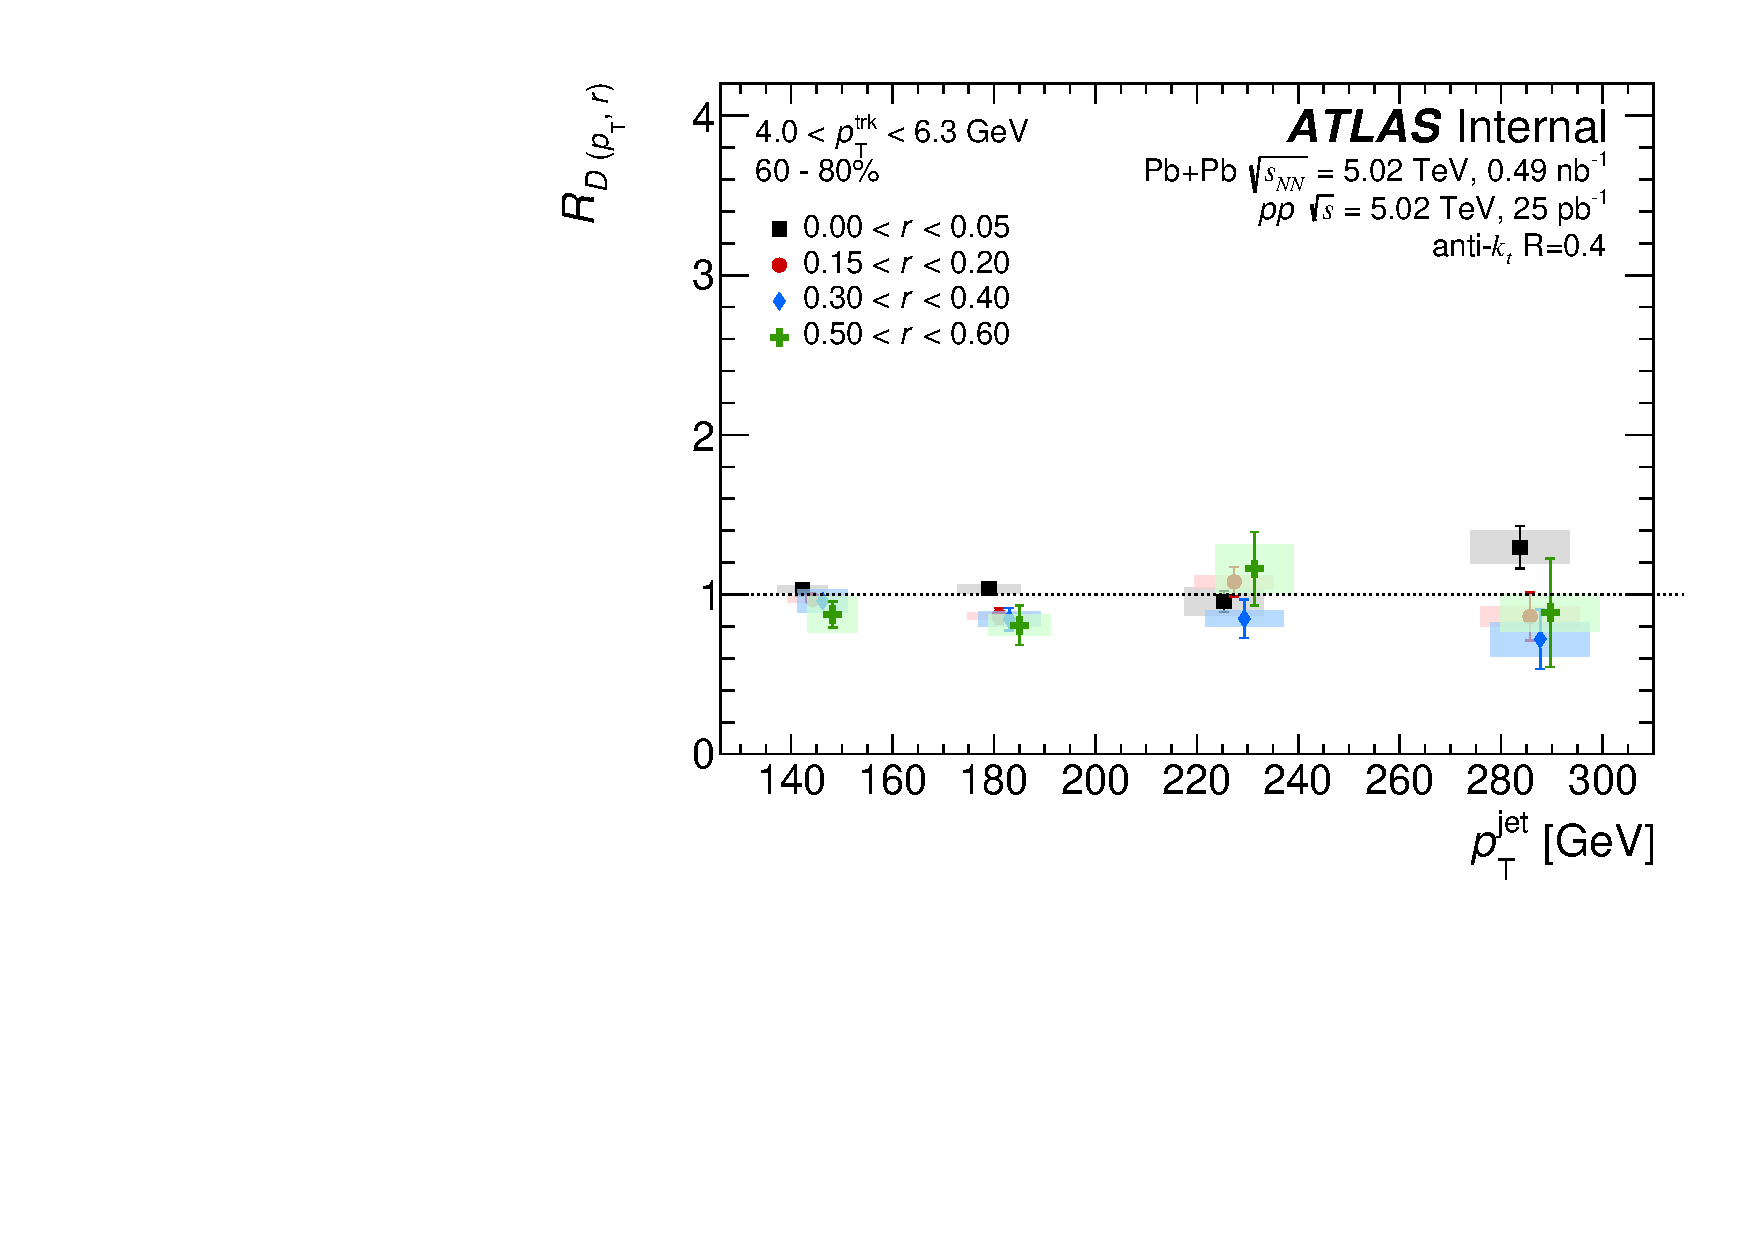
\includegraphics[width=0.45\textwidth]{results/RDpT_jetpt_trk5_cent5} \\
%\end{tabular} }
%   \caption{\RDptr as a function of \ptjet\ for charged particles with $1.0 < \pt < 1.6$ GeV (top) and $4.0 < \pt < 6.3$ GeV (bottom) at different distances from the jet axis and in 0--10\% central (left) and 60--80\% peripheral (right) \pbpb\ collisions. The vertical bars on the data points indicate statistical uncertainties while the shaded boxes indicate systematic uncertainties. The widths of the boxes are not indicative of the bin size and the points are shifted horizontally for better visibility.}
%      \label{fig:rdptr_jetpt}
%\end{figure}

%\begin{align}
%\frac{\int_1^{4} \Dpt_{\mathrm{PbPb}} \fd \pt }{\int_1^{4.2} \Dpt_{\mathrm{pp}} \fd \pt } &\qquad \frac{\int_1^{4} \Dpt_{\mathrm{PbPb}} \pt \fd \pt }{\int_1^{4} \Dpt_{\mathrm{pp}} \fd \pt } \\
%\int_1^{4} \Dpt_{\mathrm{PbPb}} - \Dpt_{\mathrm{pp}} \fd \pt  &\qquad \int_1^{4} \Dpt_{\mathrm{PbPb}} - \Dpt_{\mathrm{pp}} \pt \fd \pt \\
%\frac{\int_0^r \int_1^{4} \Dpt_{\mathrm{PbPb}} \fd \pt \fd r' }{\int_0^r \int_1^{4.2} \Dpt_{\mathrm{pp}} \fd \pt \fd r' } &\qquad \frac{\int_0^r \int_1^{4} \Dpt_{\mathrm{PbPb}} \pt \fd \pt \fd r'}{\int_0^r \int_1^{4} \Dpt_{\mathrm{pp}} \fd \pt \fd r'} \\
%\int_0^r \int_1^{4} \Dpt_{\mathrm{PbPb}} - \Dpt_{\mathrm{pp}} \fd \pt \fd dr'  &\qquad \int_0^r \int_1^{4} \Dpt_{\mathrm{PbPb}} - \Dpt_{\mathrm{pp}} \pt \fd \pt \fd dr'
%\end{align}

The measured dependence of \RDptr\ suggests that the energy lost by jets through the jet quenching process is being transferred to particles with $\pt <$~4.0~\GeV\ at larger radial distances from the jet axis. This is qualitatively consistent with theoretical calculations \mbox{\cite{Blaizot:2014ula}}.
Additionally, these observations are in agreement with the previous measurement of jet fragmentation functions \cite{Chatrchyan:2014ava, Sirunyan:2018jqr, Aaboud:2017bzv, PhysRevC.98.024908} and may indicate the dependence of the response of the hot dense matter to the momentum of a jet passing through it. 


\FloatBarrier
